\documentclass[12pt,a4paper]{article}
%\usepackage[es]{babel}
\usepackage[margin=2.5cm]{geometry}
\usepackage{graphicx}
\usepackage{xcolor}
\usepackage{fancyhdr}
\setlength{\headheight}{15pt}
\addtolength{\topmargin}{-3pt}
\usepackage{tikz}
\usepackage{array}
\usepackage{longtable}
\usepackage{hyperref}

% Color definitions
\definecolor{mainRed}{HTML}{EC3013}
\definecolor{mainGray}{HTML}{6b6866}
\definecolor{mainWhite}{HTML}{F3F2F2}

% Header and footer
\pagestyle{fancy}
\fancyhf{}
\fancyhead[C]{\textcolor{mainGray}{IEEE-830}}
\fancyfoot[C]{\thepage}
\renewcommand{\headrulewidth}{0.5pt}
\renewcommand{\headrule}{\color{mainRed}\hrule}

% Title formatting
\newcommand{\sectiontitle}[1]{%
  \section*{#1}
  \addcontentsline{toc}{section}{#1}
}

\newcommand{\subsectiontitle}[1]{%
  \subsection*{#1}
  \addcontentsline{toc}{subsection}{#1}
}

\begin{document}

% ===== PORTADA =====
\begin{titlepage}
  \centering
  \vspace*{2cm}

  {\Large\textbf{UNIVERSIDAD DISTRITAL}\\
   \textbf{FRANCISCO JOSÉ DE CALDAS}}\par

  \vspace{3cm}

  {\Huge\textbf{Especificación de Requisitos de Software}}\par

  \vspace{2cm}

  {\Large\textbf{MalphasOS}}\\
  {\large Gestión de Clientes}\par

  \vspace{3cm}

  {\large Sean Sebastián Bolívar Calderón - 20231020135}\par

  \vfill

  {\large 11 de agosto de 2026}
\end{titlepage}

% ===== TABLA DE CONTENIDOS =====
\tableofcontents
\newpage

% ===== SECCIÓN 1: INTRODUCCIÓN =====
\sectiontitle{1. Introducción}

El presente capítulo constituye el punto de partida fundamental y el marco conceptual para la Especificación de Requisitos de Software (ERS) del sistema MalphasOS. Desarrollados específicamente para la empresa BolivarBioingeniería, este documento ha sido estructurado bajo los rigurosos lineamientos de la norma internacional IEEE830 con el fin de garantizar una comunicación técnica clara, completa y sin ambigüedades entre el equipo de desarrollo, los analistas de sistemas y los diversos stakeholders del proyecto. En las secciones que conforman esta introducción, se detallará el propósito primordial del sistema orientado a la gestión integral y automatizada de clientes, así como su ámbito de aplicación, definiendo con precisión los límites de la implementación inicial (MVP) y las metas estratégicas de reducción de tiempos y errores operativos. El contenido aquí expuesto sirve como la base oficial para el diseño, desarrollo, validación y posterior puesta en marcha de la plataforma, asegurando que todas las partes involucradas compartan una visión unificada de las necesidades del negocio. Asimismo, este apartado proporciona las definiciones técnicas, acrónimos y referencias documentales necesarias para establecer un lenguaje común que facilite la trazabilidad de los requisitos.

\subsectiontitle{1.1. Propósito}

El propósito de este documento es especificar de manera clara, completa y estructurada los requisitos del sistema de gestión de clientes para la empresa BolivarBioingeniería LTDA. Este documento describe las funcionalidades, restricciones y características del sistema, sirviendo como base para su diseño, desarrollo, validación y posterior implementación. Está dirigido al equipo de desarrollo, analistas de sistemas, stakeholders del proyecto y la organización cliente, con el fin de garantizar una comprensión común de las necesidades del sistema y facilitar la comunicación entre todas las partes involucradas.

\subsectiontitle{1.2. Ámbito del sistema}

El presente apartado describe el alcance del sistema propuesto, definiendo de manera general sus funcionalidades principales, limitaciones y objetivos dentro del contexto de la empresa BolivarBioingeniería LTDA. Asimismo, se establecen los límites del sistema, identificando qué procesos serán cubiertos en su implementación inicial (MVP) y cuáles quedarán fuera de su alcance.

\subsectiontitle{1.2.1. Nombre del sistema}

El sistema propuesto se denominará \textbf{MalphasOS}: Gestión de Clientes, el cual corresponde a una plataforma de gestión de clientes orientada a optimizar los procesos operativos de la empresa BolivarBioingeniería LTDA.

\subsectiontitle{1.2.2. Alcance del Sistema}

El sistema MalphasOS estará orientado a gestionar de manera integral los procesos asociados al mantenimiento de equipos biomédicos en la empresa BolivarBioingeniería LTDA. En su versión inicial (MVP), el sistema permitirá la creación y gestión de órdenes de trabajo, la generación de reportes de mantenimiento por equipo, la administración de hojas de vida de los equipos y la captura de información en campo desde dispositivos móviles.

Asimismo, el sistema permitirá la automatización de procesos repetitivos, como la reutilización de información en reportes, la asignación automática de protocolos de mantenimiento y la firma digital de múltiples reportes en una sola operación, con el fin de mejorar la eficiencia operativa y reducir errores humanos.

Por otro lado, el sistema no contemplará en esta versión inicial funcionalidades avanzadas como la integración con sistemas externos de terceros, la gestión contable o financiera completa, el manejo de módulos complejos de facturación, el control de la vigilancia de calibraciones mediante alertas automáticas, y tampoco el manejo de inventario de las herramientas ni de los equipos patrón. Adicionalmente, funcionalidades opcionales como la generación de cotizaciones podrán estar limitadas o sujetadas a implementación futura según la priorización del proyecto.

\subsectiontitle{1.2.3. Objetivos y Beneficios esperados}

El sistema MalphasOS tiene como objetivo principal mejorar la gestión de los procesos de mantenimiento de equipos biomédicos en la empresa BolivarBioingeniería LTDA, mediante la automatización de tareas, la centralización de la información y la reducción de errores asociados a procesos manuales.

\textbf{Beneficios:}

Entre los principales beneficios esperados se encuentran la disminución del tiempo requerido para la generación de reportes de mantenimiento, la mejora en la calidad y consistencia de la información registrada, y el fortalecimiento de la trazabilidad de las intervenciones realizadas a cada equipo. Esto permitirá reducir la dependencia de procesos manuales y minimizar errores asociados a la duplicación de datos o diligenciamiento incorrecto de la información.

Adicionalmente, el sistema facilitará el trabajo en campo de los ingenieros mediante el uso de dispositivos móviles, permitiendo un registro más ágil, estructurado y en tiempo real de la información. Esto contribuirá a mejorar los tiempos operativos, facilitar la comunicación entre el personal técnico y administrativo, y asegurar que la información generada durante las actividades de mantenimiento sea completa, confiable y esté disponible de manera oportuna para su posterior análisis y uso.

\textbf{Metas:}

Se espera lograr una reducción de al menos un 40\% en el tiempo de elaboración de reportes de mantenimiento en comparación con el proceso actual, así como disminuir en un 30\% los errores asociados al diligenciamiento manual de la información. Asimismo, se busca que el 100\% de los equipos registrados cuenten con una hoja de vida digital actualizada, accesible en todo momento desde el sistema.

Adicionalmente, se plantea como meta que el sistema permita gestionar el 100\% de las órdenes de trabajo de mantenimiento preventivo dentro de la plataforma, eliminando el uso de herramientas externas como hojas de cálculo o aplicaciones de mensajería. También se espera garantizar el cumplimiento de los requisitos exigidos por las entidades regulatorias del sector salud, y mejorar la toma de decisiones operativa mediante la disponibilidad de información confiable, con tiempos de consulta inferiores a 3 segundos para reportes y datos históricos.

\subsectiontitle{1.2.4. Documentos de Referencia}

El presente documento de especificación de requisitos de software se ha elaborado siguiendo la plantilla de la norma IEEE830 y con base en la información recopilada durante el proceso de elicitación de requerimientos realizado con la empresa BolivarBioingeniería LTDA, incluyendo entrevistas, encuestas, reuniones con la gerente y un ingeniero, además del análisis de los procesos actuales y la identificación de necesidades del negocio.

Asimismo, se mantiene consistencia con los artefactos generados en etapas previas del proyecto, tales como el listado de requerimientos, listado de requisitos, la matriz de trazabilidad y los documentos de análisis del proceso de mantenimiento de equipos biomédicos. Además de los formatos que maneja la empresa para realizar las órdenes de trabajo, los mantenimientos preventivos y las hojas de vida de los equipos.

\subsectiontitle{1.3. Definiciones, Acrónimos y Abreviaturas}

En este apartado se definirán todos los términos, acrónimos y abreviaturas utilizadas en el documento de Especificación de Requisitos de Software.

\subsectiontitle{1.3.1. Definiciones}

A continuación se presentan los términos utilizados en este documento, junto con sus significados:

\begin{itemize}
  \item \textbf{Equipo biomédico:} Dispositivo utilizado en el sector salud para diagnóstico, monitoreo o tratamiento de pacientes.

  \item \textbf{Mantenimiento preventivo:} Conjunto de actividades programadas que se realizan a un equipo con el fin de prevenir fallas y garantizar su correcto funcionamiento.

  \item \textbf{Mantenimiento correctivo:} Intervención realizada para corregir fallas detectadas en un equipo.

  \item \textbf{Diagnóstico:} Proceso de evaluación de un equipo para identificar su estado y posibles fallas.

  \item \textbf{Calibración:} Proceso de comparación entre un equipo de medición y un equipo patrón para verificar la precisión de sus resultados.

  \item \textbf{Equipo patrón:} Dispositivo utilizado como referencia para realizar procesos de calibración, debido a su alta precisión certificada.

  \item \textbf{Hoja de vida del equipo:} Registro histórico que contiene toda la información relevante de un equipo, incluyendo características, mantenimientos y calibraciones realizadas.

  \item \textbf{Orden de trabajo:} Documento o registro que autoriza y describe las actividades de mantenimiento a realizar sobre uno o varios equipos.

  \item \textbf{Reporte de mantenimiento:} Documento que registra las actividades realizadas durante una intervención de mantenimiento.

  \item \textbf{Protocolo de mantenimiento:} Conjunto de procedimientos estandarizados que deben seguirse para realizar el mantenimiento de un tipo específico de equipo.
\end{itemize}

\subsectiontitle{1.3.2. Acrónimos}

A continuación se presentan los acrónimos utilizados en este documento, junto con sus significados:

\begin{itemize}
  \item \textbf{ERS} (Especificación de Requisitos de Software): Documento que describe de manera detallada los requisitos del sistema.

  \item \textbf{MVP} (Minimum Viable Product): Versión inicial del sistema que incluye únicamente las funcionalidades esenciales.

  \item \textbf{UI} (User Interface): Interfaz de usuario del sistema.

  \item \textbf{UX} (User Experience): Experiencia de usuario en la interacción con el sistema.
\end{itemize}

\subsectiontitle{1.3.3. Abreviaturas}

A continuación se presentan las abreviaturas utilizadas en este documento, junto con sus significados:

\begin{itemize}
  \item \textbf{RF:} Requisito Funcional

  \item \textbf{RNF:} Requisito No Funcional

  \item \textbf{RD:} Requisito de Dominio

  \item \textbf{BD:} Base de Datos

  \item \textbf{ID:} Identificador único
\end{itemize}

\subsectiontitle{1.4. Visión general del documento}

El presente documento de Especificación de Requisitos de Software se encuentra organizado en tres secciones principales. En la Sección 1: Introducción, se presentan el propósito del documento, el alcance del sistema, las definiciones, acrónimos y referencias utilizadas, proporcionando el contexto general del sistema propuesto.

La sección 2 aborda la descripción general del sistema, donde se describe las características globales del producto, incluyendo su perspectiva dentro del entorno organizacional, las funciones principales, las características de los usuarios, así como las restricciones, suposiciones y posibles evoluciones futuras del sistema.

Finalmente, la Sección 3 trata de los requisitos específicos, detallando de manera estructurada los requisitos del sistema, incluyendo las interfaces externas, funcionalidades, requisitos de rendimiento, restricciones de diseño y atributos del sistema, proporcionando la base para el desarrollo, validación e implementación del software.

% ===== SECCIÓN 2: DESCRIPCIÓN GENERAL =====
\newpage
\sectiontitle{2. Descripción general del documento}

En esta sección se describen los factores generales que afectan al sistema y el contexto en el que se enmarcan su desarrollo, sin entrar aún en el detalle específico de los requisitos, el cual se aborda en la Sección 3. El propósito de esta sección es proporcionar al lector una visión global del entorno operativo del sistema, así como de las condiciones, usuarios y restricciones que influyen en su funcionamiento.

Esta sección se organiza en varios apartados, en primer lugar, se presenta la perspectiva del producto, describiendo su relación con el entorno tecnológico y los procesos actuales de la empresa BolivarBioingeniería LTDA y posteriormente se ofrece un resumen de las funciones principales del sistema. Luego se detallan las características de los usuarios que interactuarán con el sistema. También se identifican las restricciones que condicionan su desarrollo e implementación, así como las suposiciones y dependencias que podrían afectar el sistema ante posibles cambios. Finalmente, se incluyen los requisitos futuros que han sido identificados, pero que no forman parte del alcance de la versión actual del sistema.

\subsectiontitle{2.1. Perspectiva del producto}

BolivarBioingeniería LTDA actualmente opera con un sistema de gestión parcial que únicamente genera reportes de mantenimiento preventivo, teniendo que complementar el proceso con hojas de vida elaboradas manualmente en Excel y un proceso de comunicación informal a través de WhatsApp entre ingenieros y personal administrativo. El nuevo sistema, denominado MalphasOS (Gestión de Clientes de BolivarBioingeniería), constituye un reemplazo y ampliación integral de este entorno fragmentado.

MalphasOS es un producto de software independiente, desarrollado a medida para BolivarBioingeniería LTDA, y no forma parte de un sistema mayor de hardware o software externo. Sin embargo, interactúa con el entorno operativo existente de la empresa en los siguientes puntos:

\begin{itemize}
  \item \textbf{Sistema actual de reportes:} MalphasOS reemplaza al programa actual de reportes, por lo que se debe contemplar la migración o consulta de los datos históricos existentes en dicho sistema y en los archivos Excel de hojas de vida, como insumo para poblar la base de datos inicial.

  \item \textbf{Dispositivos de los usuarios:} El sistema debe ser accesible desde los teléfonos celulares de los ingenieros técnicos en campo, sin necesidad de instalar aplicaciones nativas, operando como una aplicación web responsiva desde el navegador del dispositivo.

  \item \textbf{Proceso de entrega documental al cliente:} MalphasOS genera los reportes en formato PDF y Excel que actualmente se elaboran y envían manualmente, integrándose así al flujo de entrega de documentación a las entidades prestadoras de servicios de salud.
\end{itemize}

El siguiente diagrama de bloques ilustra la relación de MalphasOS con su entorno:

\begin{figure}[ht]
    \centering

    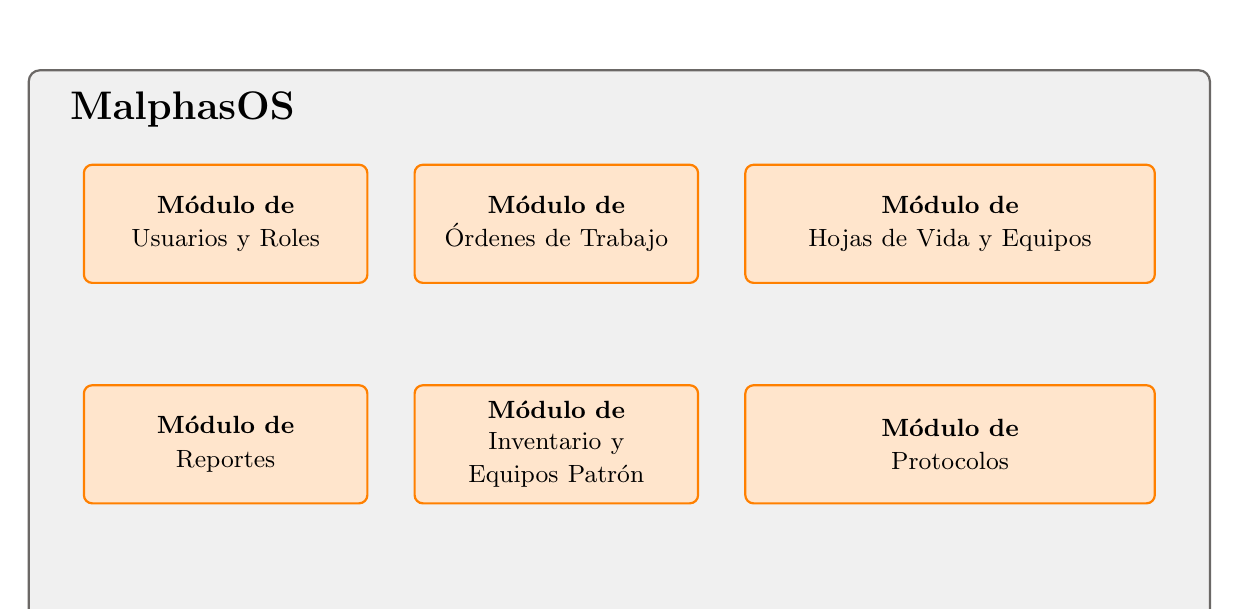
\begin{tikzpicture}

        % Contenedor principal
        \draw[
            fill=mainGray!10,
            draw=mainGray,
            thick,
            rounded corners=4pt
        ] (0,0) rectangle (15,7);

        % Título
        \node[
            anchor=west
        ] at (0.4,6.5) {
            \textbf{\Large MalphasOS}
        };

        % =====================================================
        % FILA 1
        % =====================================================

        % Usuarios y Roles
        \draw[
            fill=orange!20,
            draw=orange,
            thick,
            rounded corners=3pt
        ] (0.7,4.3) rectangle (4.3,5.8);

        \node[
            align=center,
            text width=3.1cm
        ] at (2.5,5.05) {
            \small\textbf{Módulo de}\\
            \small Usuarios y Roles
        };

        % Órdenes de Trabajo
        \draw[
            fill=orange!20,
            draw=orange,
            thick,
            rounded corners=3pt
        ] (4.9,4.3) rectangle (8.5,5.8);

        \node[
            align=center,
            text width=3.1cm
        ] at (6.7,5.05) {
            \small\textbf{Módulo de}\\
            \small Órdenes de Trabajo
        };

        % Hojas de Vida y Equipos
        \draw[
            fill=orange!20,
            draw=orange,
            thick,
            rounded corners=3pt
        ] (9.1,4.3) rectangle (14.3,5.8);

        \node[
            align=center,
            text width=4.2cm
        ] at (11.7,5.05) {
            \small\textbf{Módulo de}\\
            \small Hojas de Vida y Equipos
        };


        % =====================================================
        % FILA 2
        % =====================================================

        % Reportes
        \draw[
            fill=orange!20,
            draw=orange,
            thick,
            rounded corners=3pt
        ] (0.7,1.5) rectangle (4.3,3);

        \node[
            align=center,
            text width=3.1cm
        ] at (2.5,2.25) {
            \small\textbf{Módulo de}\\
            \small Reportes
        };

        % Inventario y Equipos Patrón
        \draw[
            fill=orange!20,
            draw=orange,
            thick,
            rounded corners=3pt
        ] (4.9,1.5) rectangle (8.5,3);

        \node[
            align=center,
            text width=3.1cm
        ] at (6.7,2.25) {
            \small\textbf{Módulo de}\\
            \small Inventario y\\
            \small Equipos Patrón
        };

        % Protocolos
        \draw[
            fill=orange!20,
            draw=orange,
            thick,
            rounded corners=3pt
        ] (9.1,1.5) rectangle (14.3,3);

        \node[
            align=center,
            text width=4.2cm
        ] at (11.7,2.25) {
            \small\textbf{Módulo de}\\
            \small Protocolos
        };

    \end{tikzpicture}

    \caption{Diagrama de Bloques de MalphasOS}
    \label{fig:bloques}

\end{figure}

\newpage

\subsectiontitle{2.2. Funciones del producto}

MalphasOS proveerá las siguientes funciones principales:

\begin{enumerate}
  \item[\textbf{a)}] \textbf{Gestión de usuarios y control de acceso.}
  El sistema permitirá la autenticación de usuarios mediante credenciales (usuario y contraseña) con identificación automática de rol. Se manejarán tres roles: SuperUsuario, Administrador e Ingeniero Técnico, cada uno con acceso restringido a las funcionalidades que le corresponden.

  \item[\textbf{b)}] \textbf{Gestión de clientes y sedes.}
  El sistema mantendrá un catálogo de clientes con toda su información institucional (nombre, NIT, dirección, ciudad, sedes, áreas de servicio y profesional responsable), el cual alimentará automáticamente los demás módulos del sistema, evitando el reingreso manual de estos datos.

  \item[\textbf{c)}] \textbf{Gestión de hojas de vida de equipos.}
  El sistema permitirá crear, consultar, modificar y mantener actualizada la hoja de vida de cada equipo hospitalario, incluyendo su identificación, características técnicas, información del fabricante, datos del servicio técnico e historial completo de intervenciones realizadas. El historial se actualizará automáticamente tras cada mantenimiento documentado.

  \item[\textbf{d)}] \textbf{Creación y gestión de órdenes de trabajo.}
  El sistema permitirá crear órdenes de trabajo directamente, sin necesidad de una solicitud previa, seleccionando el cliente, la sede, las áreas de servicio, los equipos a intervenir, el tipo de servicio y la periodicidad. Una sola orden de trabajo podrá abarcar múltiples áreas y equipos de una misma sede.

  \item[\textbf{e)}] \textbf{Generación automatizada de reportes de mantenimiento.}
  A partir de una orden de trabajo, el sistema generará automáticamente un reporte individual por cada equipo seleccionado, pre-cargado con los datos del cliente, la sede, los responsables y el protocolo de mantenimiento correspondiente al tipo de equipo y tipo de servicio. El ingeniero solo deberá completar la información técnica específica de cada intervención.

  \item[\textbf{f)}] \textbf{Gestión de protocolos de mantenimiento.}
  El sistema mantendrá un catálogo de protocolos de mantenimiento configurados por tipo de equipo y tipo de servicio, los cuales se asignarán automáticamente a cada reporte, eliminando la selección manual.

  \item[\textbf{g)}] \textbf{Firma digital unificada.}
  El sistema permitirá capturar la firma digital del cliente o responsable una sola vez por orden de trabajo, replicándola automáticamente a todos los reportes asociados a dicha intervención.

  \item[\textbf{h)}] \textbf{Exportación de documentos.}
  El sistema permitirá exportar los reportes de mantenimiento en formato PDF y Excel, con estructura consistente y formato estandarizado de BolivarBioingeniería, listos para ser entregados al cliente.

  \item[\textbf{i)}] \textbf{Gestión de inventario y equipos patrón.}
  El sistema dispondrá de un módulo de inventario para registrar y controlar equipos, herramientas y repuestos utilizados en las visitas, así como los equipos patrón utilizados en calibración, con seguimiento de su vigencia.

  \item[\textbf{j)}] \textbf{Alertas de vencimiento de calibración.}
  El sistema generará automáticamente alertas cuando la fecha de vencimiento de calibración de un equipo patrón esté dentro de los 30 días siguientes, mostrándolas en el panel principal del sistema.
\end{enumerate}

\subsectiontitle{2.3. Características de los Usuarios}

El sistema contará con tres tipos de usuarios, a continuación se explican las funciones de cada uno de los roles:

\begin{enumerate}
  \item \textbf{SuperUsuario:}
  Perfil técnico con conocimiento avanzado del sistema, es el responsable de la configuración inicial y mantenimiento de los accesos al sistema. Interactúa con el sistema ocasionalmente, principalmente para crear, modificar o eliminar cuentas de Administradores e Ingenieros. Se asume que tiene experiencia en el manejo de sistemas de información.

  \item \textbf{Administrador:}
  Personal del área administrativa de BolivarBioingeniería con nivel educativo técnico o universitario y experiencia básica en el uso de computadores y aplicaciones web. Es el usuario principal del módulo de gestión interna del sistema: gestiona el catálogo de clientes, crea y supervisa las órdenes de trabajo, configura protocolos y realiza el seguimiento de los reportes. Interactúa con el sistema diariamente, principalmente desde computador de escritorio, aunque debe poder hacerlo desde dispositivos móviles si es necesario. No se requiere experiencia técnica en software para operar el sistema.

  \item \textbf{Ingeniero Técnico:}
  Técnico o profesional en ingeniería biomédica, electrónica o afín, con experiencia en mantenimiento de equipos hospitalarios. Es el usuario de campo que accede al sistema principalmente desde su teléfono celular durante o después de las visitas de mantenimiento para consultar las órdenes de trabajo asignadas, visualizar los equipos a intervenir y registrar la información de los reportes. Su experiencia con aplicaciones de software es básica a intermedia, por lo que el sistema debe ser especialmente simple e intuitivo para este perfil. No se requiere capacitación avanzada para operar las funciones que le corresponden.
\end{enumerate}

\subsectiontitle{2.4. Restricciones}

El desarrollo e implementación de MalphasOS estará sujeto a las siguientes restricciones:

\textbf{Políticas de la empresa}

\begin{itemize}
  \item El sistema debe generar documentación que cumpla con los requisitos exigidos por la Secretaría de Salud para equipos hospitalarios, incluyendo la hoja de vida y los reportes de mantenimiento preventivo con calibración.

  \item El sistema no debe exponer información de clientes o equipos a usuarios no autorizados, dado el carácter confidencial de los datos del sector salud.
\end{itemize}

\textbf{Presupuesto y tiempo}

\begin{itemize}
  \item El presupuesto inicial disponible para el desarrollo es de quince millones de pesos colombianos (COP \$15.000.000).

  \item El tiempo estimado para la entrega del sistema es de seis meses o menos a partir del inicio del proyecto (para la realización del MVP será solo de mes y medio).
\end{itemize}

\textbf{Interfaces con otras aplicaciones}

\begin{itemize}
  \item El sistema no requiere integración automática con sistemas externos de terceros en su versión inicial. La transferencia de información desde el sistema actual se realizará mediante importación manual o migración de datos al inicio.
\end{itemize}

\textbf{Requisitos de hardware}

\begin{itemize}
  \item El sistema no requerirá de la instalación de software nativo en los dispositivos de los ingenieros, ya que deberá funcionar íntegramente desde el navegador web de dispositivos móviles con conexión a internet.
\end{itemize}

\textbf{Consideraciones de seguridad}

\begin{itemize}
  \item El acceso al sistema estará restringido mediante autenticación con usuario y contraseña.

  \item La gestión de sesiones deberá implementarse bajo el estándar JSON Web Token (JWT).

  \item Los roles de usuario definirán en precisión las funcionalidades accesibles para cada perfil, impidiendo el acceso no autorizado entre módulos.
\end{itemize}

\textbf{Capacitación}

\begin{itemize}
  \item El sistema deberá ser suficientemente intuitivo para que los ingenieros técnicos puedan operarlo con una capacitación mínima. Se contempla una sesión de capacitación formal al momento de la entrega del producto.
\end{itemize}

\subsectiontitle{2.5. Suposiciones y dependencias}

El contenido de este documento asume que los siguientes factores se mantendrán estables durante el desarrollo e implementación del sistema. Si alguno de ellos cambia, será necesario revisar los requisitos afectados.

\textbf{Suposiciones:}

\begin{itemize}
  \item Se asume que BolivarBioingeniería LTDA. continuará operando bajo el esquema actual de roles (Administrador e Ingeniero Técnico) durante la vida útil del sistema en su versión inicial.

  \item Se asume que los ingenieros técnicos disponen de teléfonos celulares con navegador web moderno (Chrome o Safari) y conexión a internet durante o después de las visitas a clientes.

  \item Se asume que la Secretaría de Salud mantendrá los requisitos actuales de documentación (hoja de vida, reportes de mantenimiento preventivo, calibraciones) sin cambios estructurales durante el desarrollo del proyecto. Un cambio regulatorio podría requerir ajustes en los modelos de datos y plantillas de reportes.

  \item Se asume que los clientes de BolivarBioingeniería seguirán siendo entidades del sector salud (IPS, hospitales, clínicas) regidas por las normas vigentes de la Secretaría de Salud.

  \item Se asume que la información de clientes y equipos existente en el sistema actual y en los archivos Excel estará disponible y en condiciones de ser migrada al nuevo sistema al inicio del proyecto.

  \item Se asume que los tipos de equipo hospitalario gestionados por la empresa (equipos básicos de consultorio, robustos/especializados, de laboratorio clínico, de terapia física y de refrigeración) no sufrirán cambios significativos en su clasificación durante el desarrollo.
\end{itemize}

\textbf{Dependencias:}

\begin{itemize}
  \item El sistema depende de la disponibilidad de infraestructura de hosting web con las características de disponibilidad requeridas (\(\geq\) 99\% en horario operativo).

  \item La funcionalidad de exportación a PDF y Excel depende de las librerías de generación de documentos seleccionadas durante el diseño técnico.

  \item La firma digital táctil depende de la compatibilidad del componente de captura con los navegadores móviles utilizados por los ingenieros.
\end{itemize}

\subsectiontitle{2.6. Requisitos futuros}

Los siguientes elementos han sido identificados como posibles mejoras al sistema para versiones futuras, y quedan fuera del alcance de la versión inicial del sistema:

\begin{itemize}
  \item \textbf{Módulo de cotizaciones:} Generación de cotizaciones de servicios de mantenimiento desde el sistema, con la posibilidad de convertir una cotización aprobada automáticamente en una orden de trabajo.

  \item \textbf{Exportación masiva de documentación:} Generación automática de carpetas de entrega al cliente con los reportes, el contrato de servicio y el cronograma de mantenimiento preventivo, empaquetados y listos para enviar.

  \item \textbf{Notificaciones push o por correo electrónico:} Envío de alertas de vencimiento de calibración y recordatorios de mantenimientos próximos directamente al correo electrónico o dispositivo del administrador.

  \item \textbf{Integración con sistemas de facturación:} Vinculación de las órdenes de trabajo completadas con el proceso de facturación de la empresa.

  \item \textbf{Cronograma de mantenimiento preventivo:} Módulo de planificación que genere y gestione automáticamente el cronograma de mantenimientos por cliente según la periodicidad requerida (semestral o anual).

  \item \textbf{Aplicación móvil nativa:} Desarrollo de una aplicación nativa para Android e iOS que permita el uso offline del sistema en campo, sincronizando la información cuando se recupere la conexión a internet.
\end{itemize}

% ===== SECCIÓN 3: REQUISITOS ESPECÍFICOS =====
\newpage
\sectiontitle{3. Requisitos Específicos}

En esta sección se presentan los requisitos del sistema con un nivel de detalle suficiente para permitir su diseño, desarrollo y validación. Los requisitos aquí definidos describen el comportamiento externo del sistema, es decir, las funcionalidades y características perceptibles por los usuarios, operadores y otros sistemas con los que interactúe.

Cada requisito ha sido formulado de manera clara y estructurada, y se encuentra identificado mediante un código único que facilita su gestión y trazabilidad a lo largo del ciclo de vida del sistema. Asimismo, los requisitos han sido organizados y clasificados según su naturaleza (funcionales, no funcionales y de dominio), permitiendo una mejor comprensión y priorización durante el desarrollo.

Para garantizar la calidad de esta especificación, los requisitos han sido definidos procurando cumplir con principios fundamentales como la claridad, la ambigüedad, la consistencia y la verificabilidad. De igual manera, se ha buscado que el documento sea fácilmente comprensible por los diferentes actores involucrados en el proyecto, incluyendo personal técnico y no técnico, y que permita realizar modificaciones y seguimiento de manera controlada mediante mecanismos de trazabilidad.

\subsectiontitle{3.1. Interfaces externas}

El sistema MalphasOS deberá interactuar con diferentes tipos de interfaces externas, incluyendo la interfaz de usuario, interfaces con dispositivos hardware y posibles interfaces de comunicación. Estas interfaces son fundamentales para garantizar la correcta interacción entre el sistema, los usuarios y el entorno operativo.

\subsectiontitle{3.1.1. Interfaz de usuario}

El sistema contará con una interfaz de usuario accesible desde navegadores web, optimizada para dispositivos móviles, especialmente teléfonos celulares, conforme a los requisitos RNF-12, RNF-13 y RNF-14, los cuales establecen la accesibilidad web, el diseño responsivo y la interacción mediante pantalla táctil.

La interfaz incluirá formularios para la gestión de órdenes de trabajo, clientes, equipos, hojas de vida, inventario y cotizaciones, de acuerdo con los requisitos RF-03, RF-08, RF-22, RF-35 y RF-45, los cuales definen la existencia de formularios para la creación y gestión de dichas entidades dentro del sistema.

Asimismo, la interfaz deberá facilitar la interacción del usuario mediante componentes como listas desplegables, autocompletado y selección múltiple, en cumplimiento del requisito RNF-16, con el objetivo de minimizar la entrada manual de datos.

El sistema también deberá permitir la visualización organizada de la información, como listados de equipos ordenados por área y tipo, según los requisitos RF-31, RF-32, RF-33 y RF-34, garantizando una presentación clara y estructurada de los datos.

Adicionalmente, el sistema deberá proporcionar mecanismos de captura de información en campo, incluyendo:

\begin{itemize}
  \item La toma de fotografías desde el dispositivo móvil (RF-28, RF-29, RF-30)

  \item La captura de firmas digitales mediante interacción táctil (RF-18, RF-21)
\end{itemize}

Estas funcionalidades permiten soportar el trabajo en campo de los usuarios y garantizar la recolección eficiente de información.

\subsectiontitle{3.1.2. Interfaces de hardware}

El sistema deberá interactuar con los siguientes componentes de hardware disponibles en los dispositivos móviles:

\begin{itemize}
  \item \textbf{Cámara del dispositivo,} utilizada para la captura de fotografías de los equipos durante las actividades de mantenimiento, conforme a los requisitos RF-28 y RF-29.

  \item \textbf{Pantalla táctil,} utilizada para la navegación del sistema y la captura de firmas digitales de los clientes o responsables, de acuerdo con los requisitos RNF-14 y RF-18.
\end{itemize}

Estas interfaces permiten la interacción directa del usuario con el sistema en entornos de trabajo en campo.

No se contemplan interfaces directas con equipos biomédicos ni con dispositivos físicos externos especializados en esta versión del sistema (MVP).

\subsectiontitle{3.1.3. Interfaces de comunicación}

El sistema operará sobre la web, requiriendo conexión a internet para el acceso a sus funcionalidades principales. La comunicación entre el navegador y el servidor se realizará mediante protocolos estándar de transferencia de datos. Asimismo, el sistema deberá permitir:

\begin{itemize}
  \item La exportación de reportes en formatos digitales como Excel (.xlsx) y PDF (.pdf), conforme a los requisitos RF-16 y RF-17, los cuales definen la generación de documentos en dichos formatos.

  \item La autenticación de usuarios mediante mecanismos seguros basados en tokens, de acuerdo con el requisito RNF-23, que establece el uso de JSON Web Token (JWT) para la gestión de sesiones.
\end{itemize}

En esta versión del sistema (MVP), no se contemplan integraciones con sistemas externos de terceros, como plataformas de facturación, sistemas hospitalarios o servicios en la nube externos.

\subsectiontitle{3.2. Funciones}

En este apartado se presentan las funciones que deberá cumplir el sistema, descritas a través de los requisitos funcionales identificados durante el proceso de análisis. Estos requisitos se han agrupado por dominio funcional, facilitando su comprensión, implementación y posterior modelado mediante diagramas de casos de uso.

Para cada dominio identificado, se detallan los requisitos funcionales asociados, especificando su identificador (ID), nombre, descripción y criterios de aceptación, así como las dependencias relevantes cuando aplique. Posteriormente, se presenta el diagrama de casos de uso correspondiente a cada dominio, el cual permite visualizar las interacciones entre los usuarios y el sistema en relación con las funcionalidades descritas. Finalmente, se incluye una breve conclusión por cada agrupación, con el fin de sintetizar el alcance funcional cubierto y su aporte dentro del sistema global.

\subsectiontitle{3.2.1. Gestión de Órdenes de Trabajo}

Este dominio agrupa las funcionalidades relacionadas con la creación, configuración y gestión de órdenes de trabajo dentro del sistema. Permite estructurar las actividades de mantenimiento mediante la selección de clientes, sedes, áreas de servicio y equipos, consolidando la información necesaria para la ejecución de las intervenciones.

\textbf{RF-01 Crear orden de trabajo directa:}

El sistema debe proporcionar una funcionalidad que permita crear registros de órdenes de trabajo de forma directa dentro del sistema.

\begin{itemize}
  \item \textbf{Nivel de Complejidad:} Alta

  \item \textbf{Criterios de Aceptación:}
  \begin{itemize}
    \item Existe un botón o acción clara para crear una nueva Orden de trabajo.
    \item La Orden de trabajo se crea sin requerir ningún registro de solicitud previo.
    \item El registro queda guardado en la base de datos con un identificador.
  \end{itemize}

  \item \textbf{Dependencias:}
  \begin{itemize}
    \item RF-49, RF-50
  \end{itemize}
\end{itemize}

\textbf{RF-02 Eliminación de dependencia de solicitud:}

El sistema no debe requerir la existencia ni la selección de registros de tipo ``solicitud'' como condición previa para la creación de una orden de trabajo.

\begin{itemize}
  \item \textbf{Nivel de Complejidad:} Baja

  \item \textbf{Criterios de Aceptación:}
  \begin{itemize}
    \item El formulario de Orden de trabajo no muestra campo obligatorio de solicitud.
    \item No se genera error al no seleccionar una solicitud previa.
    \item El flujo de creación de Orden de trabajo se completa sin solicitud.
  \end{itemize}

  \item \textbf{Dependencias:}
  \begin{itemize}
    \item RF-01
  \end{itemize}
\end{itemize}

\textbf{RF-03 Formulario de orden de trabajo:}

El sistema debe disponer de un formulario para la creación de órdenes de trabajo. El formulario debe incluir los campos Cliente, Sede, Áreas, Tipo de servicio, Periodicidad.

\begin{itemize}
  \item \textbf{Nivel de Complejidad:} Alta

  \item \textbf{Criterios de Aceptación:}
  \begin{itemize}
    \item El formulario incluye todos los campos requeridos.
    \item Cada campo tiene validación de datos.
    \item Al guardar, la Orden de trabajo queda almacenada con los datos ingresados.
  \end{itemize}

  \item \textbf{Dependencias:}
  \begin{itemize}
    \item RF-01, RF-08
  \end{itemize}
\end{itemize}

\textbf{RF-04 Selección múltiple de áreas:}

El sistema debe permitir seleccionar múltiples áreas de servicio asociadas a la sede seleccionada dentro de una misma orden de trabajo.

\begin{itemize}
  \item \textbf{Nivel de Complejidad:} Media

  \item \textbf{Criterios de Aceptación:}
  \begin{itemize}
    \item Se pueden seleccionar 2 o más áreas en una misma Orden de trabajo.
    \item Las áreas disponibles se filtran según la sede elegida.
    \item La selección múltiple se guarda correctamente.
  \end{itemize}

  \item \textbf{Dependencias:}
  \begin{itemize}
    \item RF-03, RF-08
  \end{itemize}
\end{itemize}

\textbf{RF-05 Identificador único de orden:}

El sistema debe almacenar cada orden de trabajo creada con un identificador único de tipo UUID y asociar la información ingresada en el formulario.

\begin{itemize}
  \item \textbf{Nivel de Complejidad:} Media

  \item \textbf{Criterios de Aceptación:}
  \begin{itemize}
    \item Cada Orden de trabajo generada tiene un UUID único.
    \item Todos los campos del formulario quedan persistidos en BD.
    \item El UUID se puede usar para consultar la Orden de trabajo posteriormente.
  \end{itemize}

  \item \textbf{Dependencias:}
  \begin{itemize}
    \item RF-03, RF-04, RF-07
  \end{itemize}
\end{itemize}

\textbf{RF-06 Visualización de equipos por área:}

El sistema debe mostrar los equipos disponibles organizados por cada área de servicio seleccionada dentro del formulario de creación de la orden de trabajo.

\begin{itemize}
  \item \textbf{Nivel de Complejidad:} Alta

  \item \textbf{Criterios de Aceptación:}
  \begin{itemize}
    \item Los equipos se muestran agrupados por área.
    \item Solo se muestran equipos de las áreas seleccionadas.
    \item La lista se actualiza dinámicamente al cambiar áreas.
  \end{itemize}

  \item \textbf{Dependencias:}
  \begin{itemize}
    \item RF-05, RF-09
  \end{itemize}
\end{itemize}

\textbf{RF-07 Selección múltiple de equipos:}

El sistema debe permitir seleccionar múltiples equipos pertenecientes a las áreas seleccionadas para ser incluidos en la misma orden de trabajo.

\begin{itemize}
  \item \textbf{Nivel de Complejidad:} Alta

  \item \textbf{Criterios de Aceptación:}
  \begin{itemize}
    \item Se pueden seleccionar múltiples equipos de las áreas elegidas.
    \item Solo se muestran equipos de las áreas seleccionadas.
    \item Los equipos seleccionados quedan asociados a la Orden de trabajo.
  \end{itemize}

  \item \textbf{Dependencias:}
  \begin{itemize}
    \item RF-06, RF-04
  \end{itemize}
\end{itemize}

[DIAGRAMA DE CASOS DE USO - GESTIÓN DE ÓRDENES DE TRABAJO]

\begin{figure}[h]
\centering
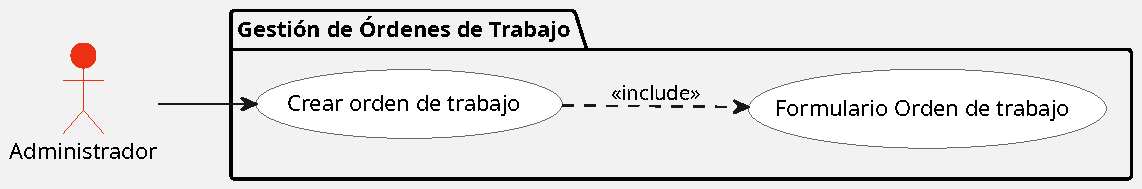
\includegraphics[width=0.95\textwidth]{use_cases/ordenes_trabajo/ordenes_trabajo.pdf}
\caption{CU - Gestión de Órdenes de Trabajo}
\label{fig:cu_ordenes_trabajo}
\end{figure}

Las funcionalidades de este dominio constituyen el eje central del sistema, ya que permiten iniciar y organizar el flujo de trabajo operativo, garantizando una adecuada planificación y trazabilidad de las actividades de mantenimiento.

\subsectiontitle{3.2.2. Gestión de Clientes}

Este dominio contempla las funcionalidades necesarias para la administración de la información de los clientes, incluyendo su registro, modificación y almacenamiento en el sistema. Esta información es fundamental para alimentar otros procesos del sistema.

\textbf{RF-08 Crear cliente:}

El sistema debe permitir crear por medio de un formulario a un cliente con los datos de Nombre del Cliente, dirección, sede, NIT, ciudad, Profesional Responsable, correo, teléfono fijo, celular, sedes y áreas. Y permitir guardarlo en la Base de Datos.

\begin{itemize}
  \item \textbf{Nivel de Complejidad:} Alta

  \item \textbf{Criterios de Aceptación:}
  \begin{itemize}
    \item El formulario incluye todos los campos listados.
    \item Los registros se guardan, editan y eliminan en BD.
    \item El cliente no representa un rol de acceso al sistema.
  \end{itemize}

  \item \textbf{Dependencias:}
  \begin{itemize}
    \item RF-49, RF-50, RF-52
  \end{itemize}
\end{itemize}

La gestión de clientes permite centralizar la información institucional, facilitando su reutilización en diferentes módulos y contribuyendo a la consistencia y reducción de errores en el manejo de datos.

\subsectiontitle{3.2.3. Reportes de Mantenimiento}

Este dominio abarca las funcionalidades orientadas a la generación, gestión y exportación de reportes de mantenimiento por cada equipo intervenido, incluyendo el registro de información técnica y la automatización de datos provenientes de la orden de trabajo.

\textbf{RF-09 Generar reporte por equipo:}

El sistema debe generar un reporte de mantenimiento individual por cada equipo seleccionado dentro de una orden de trabajo.

\begin{itemize}
  \item \textbf{Nivel de Complejidad:} Alta

  \item \textbf{Criterios de Aceptación:}
  \begin{itemize}
    \item Por cada equipo en la Orden de trabajo se genera un reporte independiente.
    \item El reporte queda asociado al equipo y a la Orden de trabajo.
    \item Se puede acceder al reporte desde la Orden de trabajo.
  \end{itemize}

  \item \textbf{Dependencias:}
  \begin{itemize}
    \item RF-05, RF-07
  \end{itemize}
\end{itemize}

\textbf{RF-11 Autocompletar datos en reporte:}

El sistema debe autocompletar en cada reporte los datos del cliente, sede, responsables y tipo de servicio a partir de la información registrada en la orden de trabajo.

\begin{itemize}
  \item \textbf{Nivel de Complejidad:} Alta

  \item \textbf{Criterios de Aceptación:}
  \begin{itemize}
    \item Los campos del reporte muestran automáticamente los datos de la Orden de trabajo.
    \item No se requiere ingreso manual de estos campos.
    \item Los datos autocompletados son consistentes con la Orden de trabajo.
  \end{itemize}

  \item \textbf{Dependencias:}
  \begin{itemize}
    \item RF-05, RF-08, RF-09
  \end{itemize}
\end{itemize}

\textbf{RF-13 Asignación automática de protocolo:}

El sistema debe seleccionar automáticamente el protocolo de mantenimiento correspondiente según el tipo de equipo y el tipo de servicio definido.

\begin{itemize}
  \item \textbf{Nivel de Complejidad:} Alta

  \item \textbf{Criterios de Aceptación:}
  \begin{itemize}
    \item Al generar el reporte, el protocolo correcto se carga automáticamente.
    \item El protocolo corresponde al tipo de equipo Y al tipo de servicio.
    \item No se requiere selección manual del protocolo.
  \end{itemize}

  \item \textbf{Dependencias:}
  \begin{itemize}
    \item RF-09, RF-14
  \end{itemize}
\end{itemize}

\textbf{RF-14 Configuración de protocolos:}

El sistema debe permitir la configuración previa de protocolos asociados a cada tipo de equipo y tipo de servicio.

\begin{itemize}
  \item \textbf{Nivel de Complejidad:} Alta

  \item \textbf{Criterios de Aceptación:}
  \begin{itemize}
    \item Existe un módulo para crear y editar protocolos.
    \item Cada protocolo se asocia a uno o más tipos de equipo y tipo de servicio.
    \item Los protocolos configurados están disponibles para asignación automática.
  \end{itemize}

  \item \textbf{Dependencias:}
  \begin{itemize}
    \item RF-22
  \end{itemize}
\end{itemize}

\textbf{RF-15 Registro de información técnica:}

El sistema debe permitir ingresar y guardar la información del reporte para cada equipo de manera independiente.

\begin{itemize}
  \item \textbf{Nivel de Complejidad:} Alta

  \item \textbf{Criterios de Aceptación:}
  \begin{itemize}
    \item El reporte tiene campos: falla reportada, diagnóstico, procedimientos, observaciones, resultado.
    \item Cada reporte se guarda de forma independiente.
    \item Los datos guardados se pueden consultar posteriormente.
  \end{itemize}

  \item \textbf{Dependencias:}
  \begin{itemize}
    \item RF-09, RF-11, RF-13
  \end{itemize}
\end{itemize}

\textbf{RF-17 Exportar a PDF:}

El sistema debe permitir exportar los reportes de mantenimiento en formato PDF (.pdf).

\begin{itemize}
  \item \textbf{Nivel de Complejidad:} Alta

  \item \textbf{Criterios de Aceptación:}
  \begin{itemize}
    \item Existe botón de exportar PDF en el reporte.
    \item El PDF generado incluye toda la información del reporte.
    \item El PDF mantiene el formato y estructura estándar de BolivarBioingeniería.
  \end{itemize}

  \item \textbf{Dependencias:}
  \begin{itemize}
    \item RF-15, RF-21
  \end{itemize}
\end{itemize}

[DIAGRAMA DE CASOS DE USO - REPORTES DE MANTENIMIENTO]

\begin{figure}[h]
\centering
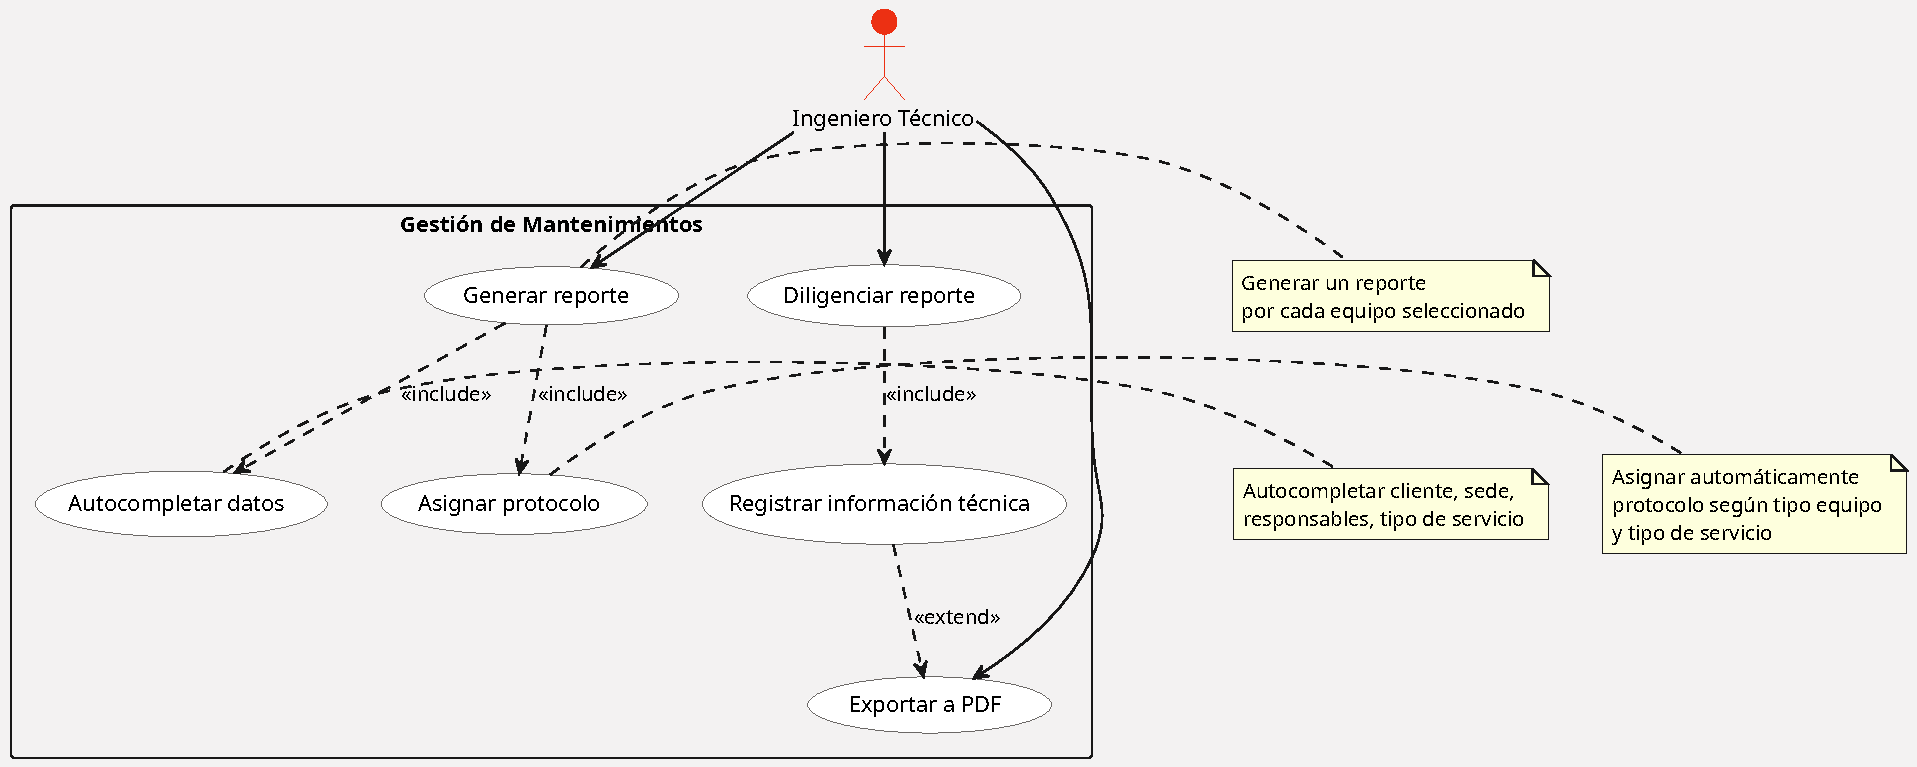
\includegraphics[width=0.95\textwidth]{use_cases/mantenimientos/mantenimientos.pdf}
\caption{CU - Gestión de Mantenimientos}
\label{fig:cu_mantenimientos}
\end{figure}

La implementación de este dominio garantiza la correcta documentación de las intervenciones realizadas, mejorando la calidad, consistencia y disponibilidad de la información generada durante los procesos de mantenimiento.

\subsectiontitle{3.2.4. Firma Digital}

Este dominio reúne las funcionalidades relacionadas con la captura, validación y aplicación de la firma digital del cliente o responsable, permitiendo formalizar la aprobación de los reportes de mantenimiento generados.

\textbf{RF-18 Captura de firma digital:}

El sistema debe permitir capturar la firma digital del cliente o responsable mediante un componente de firma táctil dentro del dispositivo móvil.

\begin{itemize}
  \item \textbf{Nivel de Complejidad:} Alta

  \item \textbf{Criterios de Aceptación:}
  \begin{itemize}
    \item El componente debe permitir al usuario dibujar su firma utilizando el dedo o un stylus en el área designada de la pantalla móvil.
    \item El componente debe mostrar el trazo de la firma en tiempo real (con un grosor de línea constante) y contar con un botón ``Borrar'' o ``Limpiar'' que elimine el trazo actual para permitir un nuevo intento.
    \item El sistema no debe permitir ``Aceptar'' o ``Finalizar'' el proceso de firma si el área del componente está vacía. Se debe mostrar un mensaje de error solicitando la firma.
  \end{itemize}

  \item \textbf{Dependencias:}
  \begin{itemize}
    \item RF-20
  \end{itemize}
\end{itemize}

\textbf{RF-21 Replicación de firma:}

El sistema debe permitir replicar la firma digital a todos los reportes de mantenimiento asociados a una misma orden de trabajo.

\begin{itemize}
  \item \textbf{Nivel de Complejidad:} Alta

  \item \textbf{Criterios de Aceptación:}
  \begin{itemize}
    \item Al capturar la firma en un reporte principal, el sistema debe replicar automáticamente la misma imagen de firma y metadatos en todos los reportes de mantenimiento vinculados al ID de la misma orden de trabajo.
    \item Antes de realizar la replicación, el sistema debe mostrar un mensaje de confirmación o un checkbox que indique: ``Deseo aplicar esta firma a todos los reportes de esta Orden de Trabajo''.
    \item El sistema debe validar que todos los reportes pertenezcan efectivamente a la misma orden OT antes de ejecutar la copia, evitando la replicación accidental en documentos ajenos.
  \end{itemize}

  \item \textbf{Dependencias:}
  \begin{itemize}
    \item RF-18
  \end{itemize}
\end{itemize}

[DIAGRAMA DE CASOS DE USO - FIRMA DIGITAL]

\begin{figure}[h]
\centering
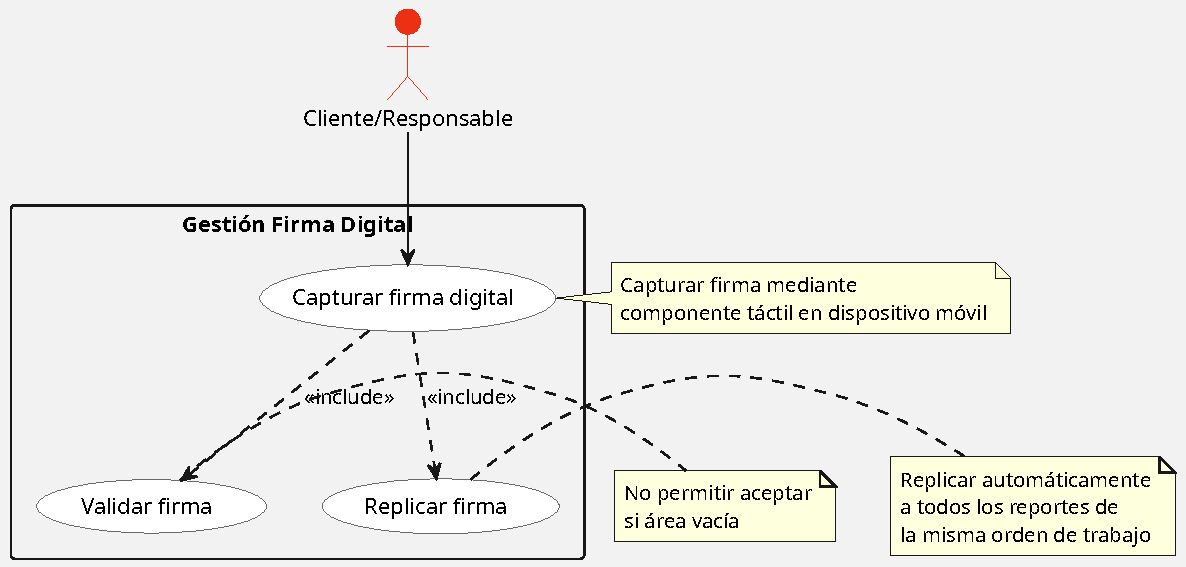
\includegraphics[width=0.95\textwidth]{use_cases/firma_digital/firma_digital.pdf}
\caption{CU - Gestión de Firma Digital}
\label{fig:cu_firma_digital}
\end{figure}

La firma digital asegura la validación de la información registrada, optimizando el proceso de aprobación y reduciendo la necesidad de procedimientos manuales o documentación física.

\subsectiontitle{3.2.5. Hojas de Vida de los Equipos}

Este dominio comprende las funcionalidades destinadas a la creación, consulta, actualización y mantenimiento de la hoja de vida de cada equipo, incluyendo su información técnica, historial de intervenciones y documentación asociada.

\textbf{RF-22 Crear hoja de vida:}

El sistema debe disponer de un formulario para la creación de la hoja de vida de un equipo.

\begin{itemize}
  \item \textbf{Nivel de Complejidad:} Alta

  \item \textbf{Criterios de Aceptación:}
  \begin{itemize}
    \item Existe un formulario de hoja de vida accesible desde el módulo de equipos.
    \item El formulario incluye todas las secciones requeridas (identificación, técnica, fabricante, servicio técnico).
    \item Al guardar, la hoja de vida queda registrada en BD.
  \end{itemize}

  \item \textbf{Dependencias:}
  \begin{itemize}
    \item RF-08, RF-49, RF-50
  \end{itemize}
\end{itemize}

\textbf{RF-24 Modificar/eliminar hoja de vida:}

El sistema debe permitir modificar y eliminar la información registrada en la hoja de vida de un equipo.

\begin{itemize}
  \item \textbf{Nivel de Complejidad:} Media

  \item \textbf{Criterios de Aceptación:}
  \begin{itemize}
    \item Existe opción de edición de la hoja de vida.
    \item Los cambios se guardan correctamente en BD.
    \item La eliminación requiere confirmación y está restringida por rol.
  \end{itemize}

  \item \textbf{Dependencias:}
  \begin{itemize}
    \item RF-22
  \end{itemize}
\end{itemize}

\textbf{RF-26 Registro automático de intervenciones:}

El sistema debe registrar automáticamente cada mantenimiento, calibración o diagnóstico realizado a un equipo en su hoja de vida.

\begin{itemize}
  \item \textbf{Nivel de Complejidad:} Alta

  \item \textbf{Criterios de Aceptación:}
  \begin{itemize}
    \item Al completar un reporte, la intervención se registra automáticamente en la hoja de vida.
    \item No se requiere acción manual para actualizar el historial.
    \item El registro incluye fecha, tipo de servicio y resultado.
  \end{itemize}

  \item \textbf{Dependencias:}
  \begin{itemize}
    \item RF-09, RF-15, RF-22
  \end{itemize}
\end{itemize}

\textbf{RF-27 Historial de intervenciones:}

El sistema debe almacenar el historial de intervenciones con información de fecha, tipo de servicio y resultado.

\begin{itemize}
  \item \textbf{Nivel de Complejidad:} Media

  \item \textbf{Criterios de Aceptación:}
  \begin{itemize}
    \item Cada entrada del historial contiene: fecha de servicio, tipo (preventivo/correctivo/etc.) y resultado (apto/no apto).
    \item El historial es consultable y ordenado cronológicamente.
    \item La información es consistente con el reporte correspondiente.
  \end{itemize}

  \item \textbf{Dependencias:}
  \begin{itemize}
    \item RF-26
  \end{itemize}
\end{itemize}

[DIAGRAMA DE CASOS DE USO - HOJAS DE VIDA]

\begin{figure}[h]
\centering
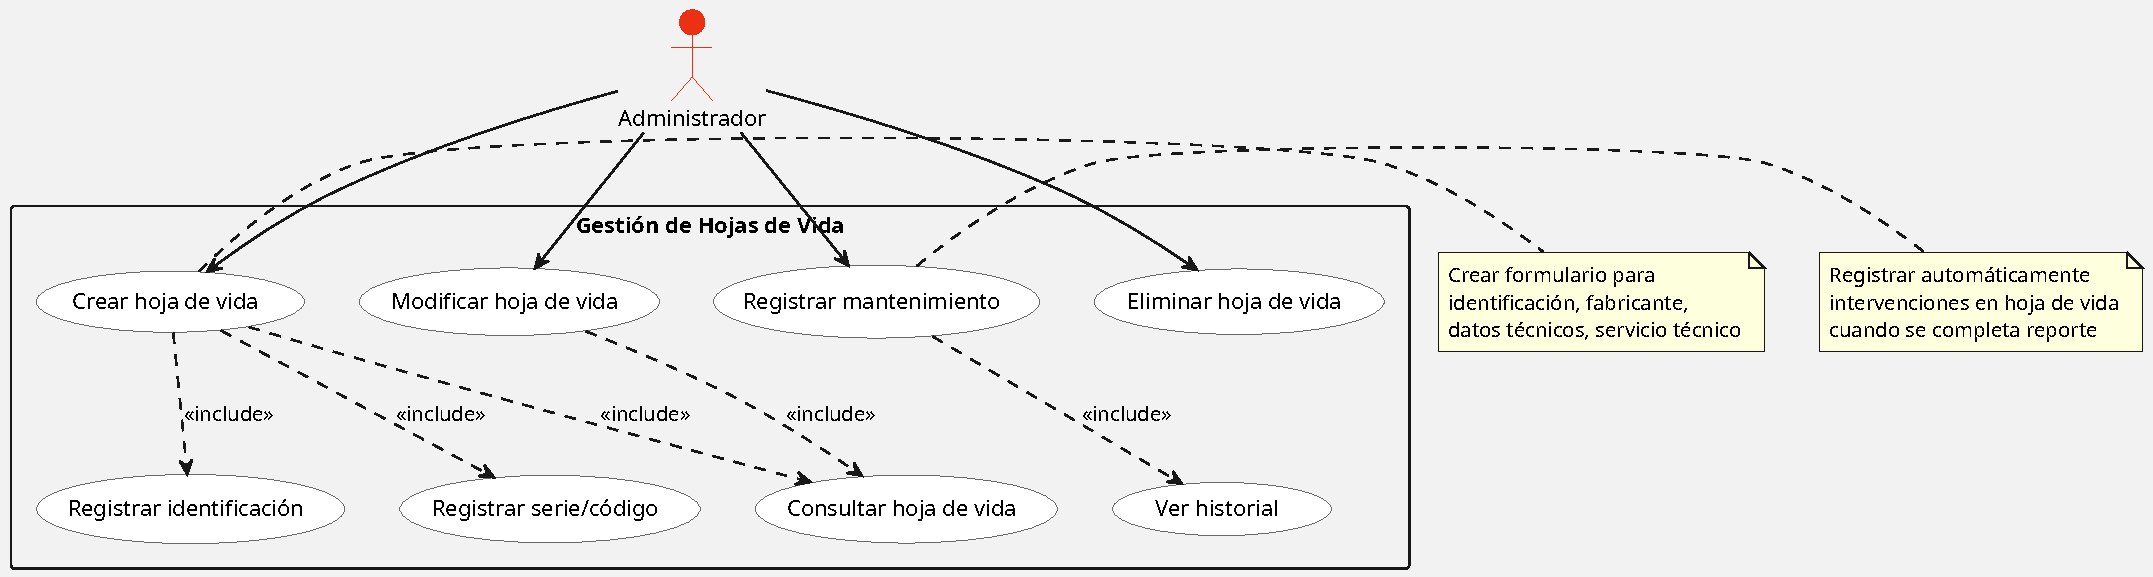
\includegraphics[width=0.95\textwidth]{use_cases/hojas_vida/hojas_vida.pdf}
\caption{CU - Gestión de Hojas de Vida}
\label{fig:cu_hojas_vida}
\end{figure}

La gestión de hojas de vida permite mantener un registro histórico completo y actualizado de cada equipo, fortaleciendo la trazabilidad y facilitando la toma de decisiones basadas en el estado y comportamiento de los equipos.

\subsectiontitle{3.2.6. Inventario}

Este dominio agrupa las funcionalidades necesarias para la gestión del inventario de equipos, herramientas y repuestos, así como el registro y control de los equipos patrón utilizados en procesos de calibración.

\textbf{RF-36 Módulo inventario:}

El sistema debe permitir registrar nuevos ítems en el inventario mediante un formulario con los campos: Nombre del ítem, Tipo (equipo, herramienta, repuesto), Cantidad disponible, Estado

\begin{itemize}
  \item \textbf{Nivel de Complejidad:} Media

  \item \textbf{Criterios de Aceptación:}
  \begin{itemize}
    \item El sistema no debe permitir guardar el registro si alguno de los campos (Nombre, Tipo, Cantidad, Estado) está vacío, resultando en campos incompletos en rojo.
    \item El campo ``Tipo'' debe ser un menú desplegable (dropdown) que permita seleccionar exclusivamente una de las tres opciones: Equipo, Herramienta o Repuesto.
    \item El sistema debe validar que el ``Nombre del ítem'' no exista previamente en el inventario para el mismo ``Tipo'', enviando una alerta si se intenta registrar un ítem duplicado.
  \end{itemize}

  \item \textbf{Dependencias:}
  \begin{itemize}
    \item RF-35
  \end{itemize}
\end{itemize}

\textbf{RF-37 Entrada/salida inventario:}

El sistema debe permitir registrar la salida y entrada de ítems del inventario durante las actividades de mantenimiento.

\begin{itemize}
  \item \textbf{Nivel de Complejidad:} Media

  \item \textbf{Criterios de Aceptación:}
  \begin{itemize}
    \item El sistema no debe permitir registrar la salida de una cantidad superior a la ``Cantidad disponible'' actual del ítem. Debe mostrar un mensaje de ``Stock insuficiente''.
    \item Al confirmar una salida, el sistema debe restar automáticamente la cantidad del inventario general; al confirmar una entrada (devolución), debe sumarla.
    \item El sistema debe capturar automáticamente el ID del usuario que realiza el movimiento de los ítems.
  \end{itemize}

  \item \textbf{Dependencias:}
  \begin{itemize}
    \item RF-35
  \end{itemize}
\end{itemize}

[DIAGRAMA DE CASOS DE USO - INVENTARIO]

\begin{figure}[h]
\centering
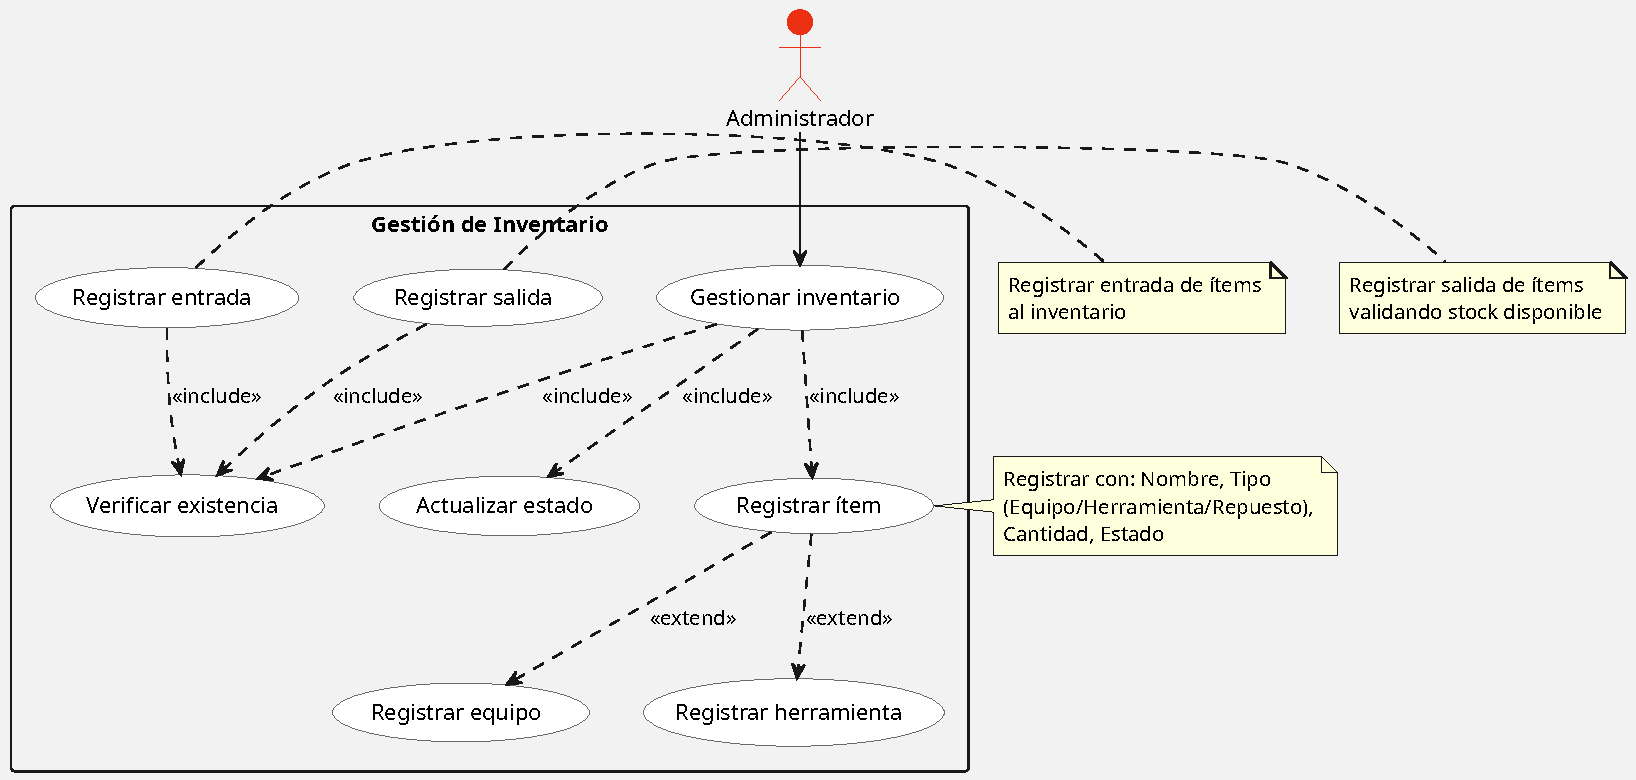
\includegraphics[width=0.95\textwidth]{use_cases/inventario/inventario.pdf}
\caption{CU - Gestión de Inventario}
\label{fig:cu_inventario}
\end{figure}

La gestión de inventario permite un control eficiente de los recursos utilizados en mantenimiento, asegurando su disponibilidad, trazabilidad y correcto uso dentro de las actividades operativas.

\subsectiontitle{3.2.7. Alertas y calibración}

Este dominio contempla las funcionalidades encargadas de monitorear el estado de calibración de los equipos patrón y generar alertas automáticas ante próximos vencimientos.

\textbf{RF-40 Identificar vencimientos:}

El sistema debe identificar automáticamente los equipos patrón cuya fecha de vencimiento de calibración esté próxima a cumplirse.

\begin{itemize}
  \item \textbf{Nivel de Complejidad:} Media

  \item \textbf{Criterios de Aceptación:}
  \begin{itemize}
    \item El sistema debe comparar diariamente la ``Fecha de última calibración'' y la ``Frecuencia de calibración'' contra la fecha actual para determinar los días restantes de vigencia.
    \item En el listado de inventario, los equipos próximos a vencer deben mostrar un indicador visual distintivo para diferenciarlos de los equipos vigentes o vencidos.
    \item El sistema debe mostrar un mensaje de advertencia si un técnico intenta asociar un equipo patrón próximo a vencer (o ya vencido) a un reporte de mantenimiento.
  \end{itemize}

  \item \textbf{Dependencias:}
  \begin{itemize}
    \item RF-11
  \end{itemize}
\end{itemize}

\textbf{RF-41 Generar alertas:}

El sistema debe generar una alerta cuando la fecha de vencimiento de calibración de un equipo patrón esté dentro de un umbral de 30 días previos.

\begin{itemize}
  \item \textbf{Nivel de Complejidad:} Media

  \item \textbf{Criterios de Aceptación:}
  \begin{itemize}
    \item Al cumplirse el umbral de 30 días, el registro del equipo debe cambiar automáticamente su estado visual a ``Alerta de Calibración'' en todos los módulos donde sea visible.
    \item La alerta debe permanecer activa y visible de forma permanente hasta que se registre un nuevo certificado de calibración que actualice la fecha de vencimiento a un período futuro.
    \item El sistema debe descontar correctamente los días considerando meses de 28, 30 y 31 días, asegurando que el cálculo sea exacto respecto al calendario gregoriano.
  \end{itemize}

  \item \textbf{Dependencias:}
  \begin{itemize}
    \item RF-40
  \end{itemize}
\end{itemize}

[DIAGRAMA DE CASOS DE USO - ALERTAS Y CALIBRACIÓN]

\begin{figure}[h]
\centering
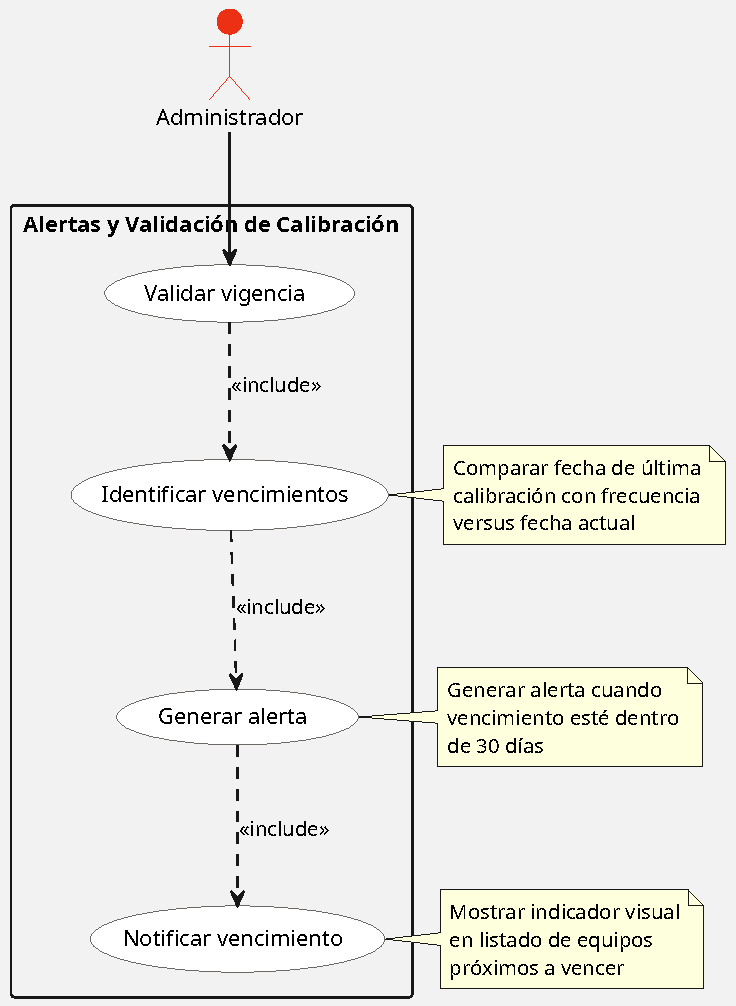
\includegraphics[width=0.95\textwidth]{use_cases/alertas_calibracion/alertas_calibracion.pdf}
\caption{CU - Alertas y Calibración}
\label{fig:cu_alertas_calibracion}
\end{figure}

Las alertas de calibración contribuyen a la prevención de errores operativos, garantizando el uso de equipos patrón vigentes y apoyando el cumplimiento de las normas regulatorias del sector salud.

\subsectiontitle{3.2.8. Módulo Comercial}

Este dominio incluye las funcionalidades orientadas a la generación y gestión de cotizaciones de servicios de mantenimiento, así como su integración con el proceso operativo mediante la creación de órdenes de trabajo.

\textbf{RF-45 Crear cotización:}

El sistema debe disponer de un formulario para la creación de cotizaciones de servicios de mantenimiento.

\begin{itemize}
  \item \textbf{Nivel de Complejidad:} Alta

  \item \textbf{Criterios de Aceptación:}
  \begin{itemize}
    \item El formulario debe permitir seleccionar un Cliente (desde una lista existente) y registrar datos básicos como: fecha de emisión, validez de la oferta (días) y moneda.
    \item El formulario debe incluir un campo para aplicar descuentos, ya sea por porcentaje (\%) o por monto fijo (\$), recalculando el total de forma inmediata.
    \item Los campos de precio y cantidad solo deben aceptar valores numéricos positivos. El sistema debe impedir el guardado si hay líneas con valores en cero o negativos.
  \end{itemize}

  \item \textbf{Dependencias:}
  \begin{itemize}
    \item RF-46
  \end{itemize}
\end{itemize}

\textbf{RF-47 Generar orden desde cotización:}

El sistema debe permitir generar una orden de trabajo a partir de una cotización en estado ``aprobada''.

\begin{itemize}
  \item \textbf{Nivel de Complejidad:} Alta

  \item \textbf{Criterios de Aceptación:}
  \begin{itemize}
    \item Al generar la OT, el sistema debe heredar automáticamente el Cliente, la lista de servicios, las cantidades y las notas técnicas de la cotización original sin requerir reingreso de datos.
    \item Una vez generada la OT, la cotización debe cambiar automáticamente a un estado final para evitar que se generen múltiples órdenes de trabajo desde la misma cotización.
    \item Al convertir la cotización, el sistema debe verificar que los repuestos incluidos sigan teniendo stock disponible. En caso de faltantes, debe mostrar una advertencia, pero permitir la creación de la Orden de trabajo como ``Pendiente de Suministros''.
  \end{itemize}

  \item \textbf{Dependencias:}
  \begin{itemize}
    \item RF-45
  \end{itemize}
\end{itemize}

[DIAGRAMA DE CASOS DE USO - MÓDULO COMERCIAL]

\begin{figure}[h]
\centering
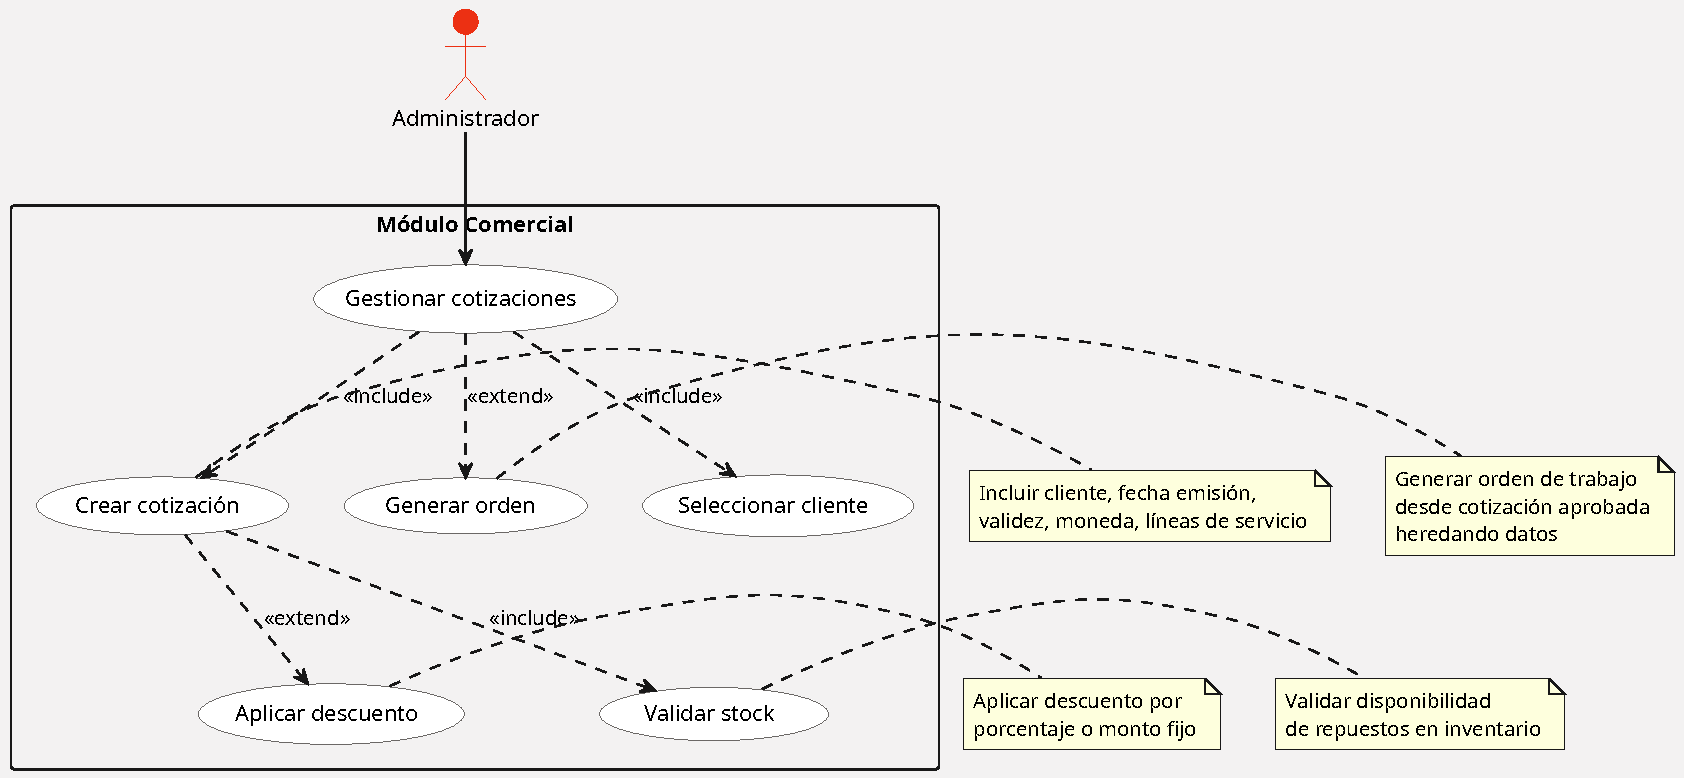
\includegraphics[width=0.95\textwidth]{use_cases/modulo_comercial/modulo_comercial.pdf}
\caption{CU - Módulo Comercial}
\label{fig:cu_modulo_comercial}
\end{figure}

El módulo comercial permite extender el alcance del sistema hacia la gestión de oportunidades de negocio, facilitando la transición entre la cotización y la ejecución del servicio.

\subsectiontitle{3.2.9. Usuarios y seguridad}

Este dominio abarca las funcionalidades relacionadas con la autenticación, autorización y gestión de usuarios del sistema, incluyendo la administración de roles y credenciales.

\textbf{RF-49 Login de usuario:}

El sistema debe permitir al usuario ingresar a la aplicación por medio de sus credenciales compuestos por usuario y contraseña.

\begin{itemize}
  \item \textbf{Nivel de Complejidad:} Alta

  \item \textbf{Criterios de Aceptación:}
  \begin{itemize}
    \item Existe pantalla de login con campos usuario y contraseña.
    \item Credenciales correctas $\rightarrow$ acceso al sistema.
    \item Credenciales incorrectas $\rightarrow$ mensaje de error sin detallar cuál campo falló.
  \end{itemize}

  \item \textbf{Dependencias:}
  \begin{itemize}
    \item RF-49
  \end{itemize}
\end{itemize}

\textbf{RF-50 Identificación de rol:}

El sistema debe poder identificar el rol dependiendo de las credenciales ingresadas por el usuario.

\begin{itemize}
  \item \textbf{Nivel de Complejidad:} Alta

  \item \textbf{Criterios de Aceptación:}
  \begin{itemize}
    \item Tras el login, el sistema identifica si el usuario es SuperUsuario, Administrador o Ingeniero.
    \item Cada rol accede solo a sus funcionalidades habilitadas.
    \item El rol incorrecto no puede acceder a funciones restringidas.
  \end{itemize}

  \item \textbf{Dependencias:}
  \begin{itemize}
    \item RF-49
  \end{itemize}
\end{itemize}

\textbf{RF-51 Creación de usuarios:}

El sistema debe permitir crear nuevos usuarios del sistema.

\begin{itemize}
  \item \textbf{Nivel de Complejidad:} Alta

  \item \textbf{Criterios de Aceptación:}
  \begin{itemize}
    \item Existe interfaz para crear nuevos usuarios con usuario, contraseña y rol asignado.
    \item Los registros se guardan en BD.
    \item El nuevo usuario puede iniciar sesión con sus credenciales.
  \end{itemize}

  \item \textbf{Dependencias:}
  \begin{itemize}
    \item RF-50
  \end{itemize}
\end{itemize}

\textbf{RF-52 Modificación de usuarios:}

El sistema debe permitir modificar y eliminar la información registrada en la cuenta de usuario.

\begin{itemize}
  \item \textbf{Nivel de Complejidad:} Media

  \item \textbf{Criterios de Aceptación:}
  \begin{itemize}
    \item Existe opción de edición de datos del usuario.
    \item Los cambios se guardan correctamente en BD.
    \item La eliminación requiere confirmación y está restringida por rol.
  \end{itemize}

  \item \textbf{Dependencias:}
  \begin{itemize}
    \item RF-50
  \end{itemize}
\end{itemize}

\textbf{RF-53 Eliminación de usuarios:}

El sistema debe permitir eliminar usuarios del sistema.

\begin{itemize}
  \item \textbf{Nivel de Complejidad:} Media

  \item \textbf{Criterios de Aceptación:}
  \begin{itemize}
    \item Existe opción de eliminación de usuario.
    \item Se requiere confirmación antes de proceder.
    \item El acceso se revoca inmediatamente.
  \end{itemize}

  \item \textbf{Dependencias:}
  \begin{itemize}
    \item RF-50
  \end{itemize}
\end{itemize}

[DIAGRAMA DE CASOS DE USO - USUARIOS Y SEGURIDAD]

\begin{figure}[h]
\centering
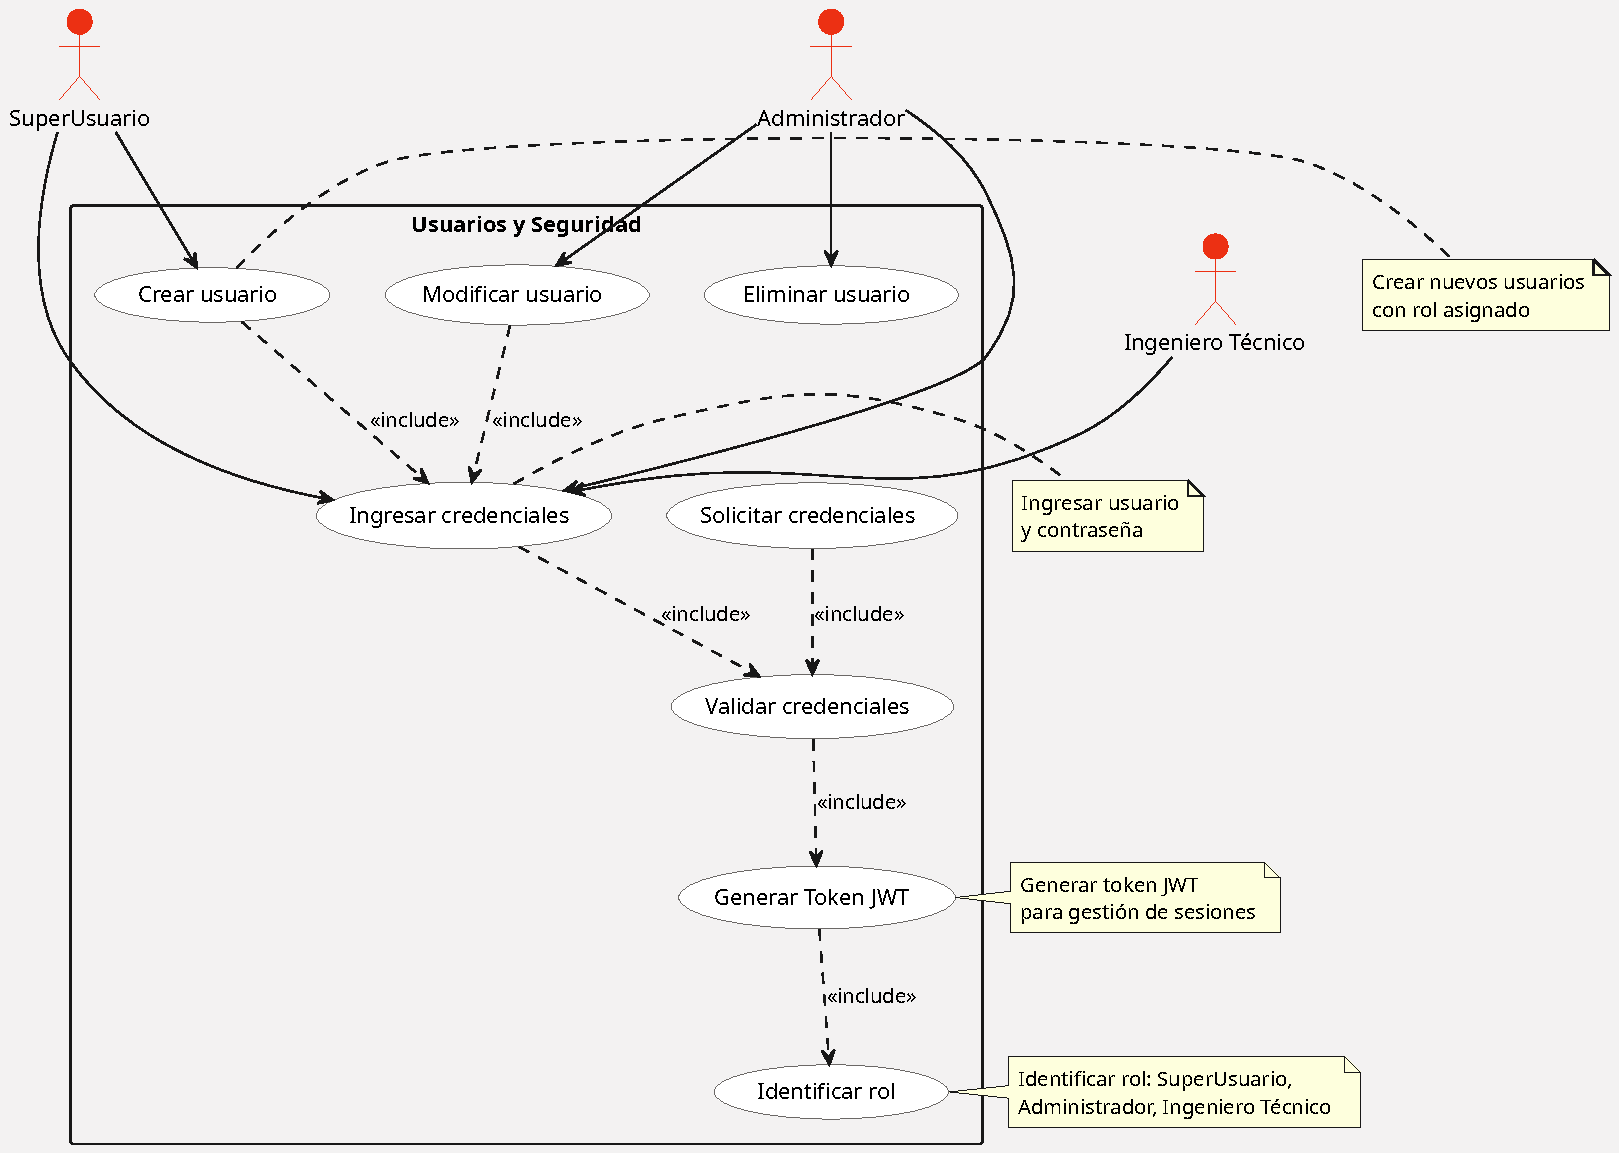
\includegraphics[width=0.95\textwidth]{use_cases/usuarios_seguridad/usuarios_seguridad.pdf}
\caption{CU - Usuarios y Seguridad}
\label{fig:cu_usuarios_seguridad}
\end{figure}

La gestión de usuarios y seguridad garantiza el acceso controlado al sistema, protegiendo la información y asegurando que cada usuario interactúe únicamente con las funcionalidades correspondientes a su rol.

\subsectiontitle{3.3. Requisitos de rendimiento}

En esta sección se describen los requisitos relacionados con el desempeño del sistema, incluyendo tiempos de respuesta, capacidad de procesamiento, concurrencia de usuarios y comportamiento frente al manejo de datos. Estos requisitos garantizan que el sistema MalphasOS opere de manera eficiente, garantizando tiempos de respuesta adecuados, alta disponibilidad y capacidad suficiente para soportar las operaciones diarias de la organización.

\textbf{RNF-01 – Tiempo de diligenciamiento de orden de trabajo:}

El sistema debe permitir que un usuario complete el formulario de creación de una orden de trabajo en un tiempo máximo de 3 minutos, sin requerir capacitación avanzada.

\begin{itemize}
  \item \textbf{Nivel de Complejidad:} Media
\end{itemize}

\textbf{RNF-03 – Tiempo de registro de orden:}

El sistema debe registrar y guardar una orden de trabajo en un tiempo máximo de 2 segundos después de que el usuario confirme la operación.

\begin{itemize}
  \item \textbf{Nivel de Complejidad:} Alta
\end{itemize}

\textbf{RNF-04 – Tiempo de carga de equipos:}

El sistema debe mostrar la lista de equipos asociados a las áreas seleccionadas en un tiempo máximo de 2 segundos después de realizar la selección.

\begin{itemize}
  \item \textbf{Nivel de Complejidad:} Alta
\end{itemize}

\textbf{RNF-09 – Tiempo de carga de reportes:}

El sistema debe cargar la lista de reportes asociados en un tiempo máximo de 2 segundos.

\begin{itemize}
  \item \textbf{Nivel de Complejidad:} Alta
\end{itemize}

\textbf{RNF-10 – Actualización de historial de equipos:}

El sistema debe actualizar el historial del equipo en un tiempo máximo de 2 segundos después de registrar una intervención.

\begin{itemize}
  \item \textbf{Nivel de Complejidad:} Alta
\end{itemize}

\textbf{RNF-18 – Actualización de inventario:}

El sistema debe reflejar la actualización del inventario en un tiempo máximo de 2 segundos después de registrar una operación.

\begin{itemize}
  \item \textbf{Nivel de Complejidad:} Media
\end{itemize}

\textbf{RNF-19 – Frecuencia de monitoreo de alertas:}

El sistema debe monitorear las alertas automáticamente al menos una vez cada 24 horas.

\begin{itemize}
  \item \textbf{Nivel de Complejidad:} Media
\end{itemize}

\textbf{RNF-20 – Tiempo de registro de reportes:}

El sistema debe permitir completar el registro de un reporte de mantenimiento por equipo en un tiempo máximo de 3 minutos.

\begin{itemize}
  \item \textbf{Nivel de Complejidad:} Alta
\end{itemize}

\textbf{RNF-21 – Disponibilidad del sistema:}

El sistema deberá estar disponible al menos el 99\% del tiempo durante el horario operativo, garantizando el registro continuo de información sin interrupciones que afecten las actividades de mantenimiento.

\begin{itemize}
  \item \textbf{Nivel de Complejidad:} Alta
\end{itemize}

\textbf{RNF-22 – Tiempo de generación de órdenes desde cotización:}

El sistema debe generar la orden de trabajo a partir de una cotización en un tiempo máximo de 2 segundos.

\begin{itemize}
  \item \textbf{Nivel de Complejidad:} Media
\end{itemize}

\textbf{Capacidad del sistema y concurrencia:}

El sistema está diseñado para ser utilizado principalmente por personal técnico y administrativo de la empresa, por lo que se estima:

\begin{itemize}
  \item \textbf{Usuarios concurrentes esperados:} entre 5 y 20 usuarios simultáneos.

  \item \textbf{Dispositivos:} principalmente dispositivos móviles y navegadores web.
\end{itemize}

\textbf{Tipo de carga:} transaccional ligera (formularios, consultas y generación de reportes).

El sistema deberá mantener los tiempos de respuesta definidos en los requisitos anteriores bajo estas condiciones de uso.

\textbf{Requisitos de datos:}

En cuanto al manejo de información, se establecen las siguientes consideraciones:

\begin{itemize}
  \item El sistema deberá soportar el almacenamiento de miles de registros asociados a:
  \begin{itemize}
    \item Órdenes de trabajo.
    \item Reportes de mantenimiento.
    \item Hojas de vida de equipos.
    \item Inventario
  \end{itemize}

  \item La frecuencia de acceso a los datos será alta, especialmente en:
  \begin{itemize}
    \item Consulta de órdenes.
    \item Registro de reportes en campo.
    \item Visualización de equipos.
  \end{itemize}

  \item El acceso a la información deberá ser rápido y consistente, garantizando tiempos de consulta inferiores a 3 segundos, en concordancia con los otros requisitos del sistema.
\end{itemize}

Los requisitos de rendimiento definidos aseguran que el sistema MalphasOS opere de manera eficiente, garantizando tiempos de respuesta adecuados, alta disponibilidad y capacidad suficiente para soportar las operaciones diarias de la organización. Estos requisitos son fundamentales para mantener la productividad de los usuarios, especialmente en entornos de trabajo en campo donde la rapidez y confiabilidad del sistema son críticas.

\subsectiontitle{3.4. Restricciones de diseño}

En esta sección se describen las restricciones que condicionan las decisiones de diseño y desarrollo del sistema MalphasOS. Estas limitaciones provienen de factores técnicos, organizacionales, normativos y operativos que deben ser considerados para garantizar la viabilidad e implementación adecuada del sistema.

\textbf{Restricciones tecnológicas:}

El sistema deberá ser desarrollado como una aplicación web, accesible desde navegadores sin requerir la instalación de software adicional en los dispositivos de los usuarios. Esto implica que el diseño deberá ajustarse a tecnologías web estándar y garantizar compatibilidad con navegadores modernos.

Asimismo, la gestión de sesiones deberá implementarse utilizando el estándar JSON Web Token (JWT), lo cual condiciona el diseño de los mecanismos de autenticación y autorización del sistema.

\textbf{Restricciones de hardware:}

El sistema deberá operar principalmente en dispositivos móviles, especialmente teléfonos celulares utilizados por los ingenieros técnicos en campo. Por lo tanto, el diseño de la interfaz deberá ser responsivo y adaptarse a diferentes tamaños de pantalla, así como soportar la interacción mediante pantalla táctil.

Adicionalmente, el sistema deberá hacer uso de los componentes de hardware disponibles en los dispositivos, tales como:

\begin{itemize}
  \item Cámara, para la captura de fotografías de los equipos.

  \item Pantalla táctil, para la interacción y captura de firmas digitales.
\end{itemize}

Estas restricciones implican que el sistema debe ser compatible con las capacidades estándar de los dispositivos móviles sin requerir hardware especializado.

\textbf{Restricciones de comunicación:}

El sistema dependerá de una conexión a internet para su funcionamiento, ya que operará como una aplicación web. Esto implica que el diseño debe considerar posibles limitaciones de conectividad en entornos de campo, optimizando el uso de recursos y minimizando tiempos de carga.

En esta versión del sistema (MVP), no se contemplan integraciones automáticas con sistemas externos de terceros, lo que restringe el diseño a un sistema autónomo.

\textbf{Restricciones de diseño de interfaz:}

El sistema deberá ser intuitivo, simple y ágil, minimizando la cantidad de pasos necesarios para realizar cada proceso o facilitando su uso por usuarios con niveles básicos o intermedios de experiencia tecnológica. Para esto, el diseño de la interfaz deberá incluir:

\begin{itemize}
  \item Componentes como listas desplegables, autocompletado y selección múltiple.

  \item Mensajes de error claros y comprensibles.

  \item Navegación optimizada para dispositivos móviles.
\end{itemize}

Estas restricciones impactan directamente en la arquitectura de la interfaz de usuario (UI) y en la experiencia de usuario (UX).

Las restricciones de diseño establecidas definen el marco dentro del cual debe desarrollarse el sistema MalphasOS, condicionando tanto las decisiones tecnológicas como la arquitectura y la experiencia de usuario. Su cumplimiento garantiza que el sistema sea viable, accesible, seguro y alineado con las necesidades operativas y regulatorias de la organización.

\subsectiontitle{3.5. Priorización MoSCoW}

Con el fin de establecer una estrategia de desarrollo alineada con las necesidades de BolivarBioingeniería LTDA. y las restricciones de tiempo y presupuesto definidas para el proyecto, los requisitos del sistema fueron priorizados con la gerente de la empresa utilizando la metodología MoSCoW. Esta técnica permite clasificar los requisitos de acuerdo con su importancia y su inclusión dentro del Producto Mínimo Viable (MVP).

La clasificación realizada permitió definir el alcance del MVP de MalphasOS, priorizando las funcionalidades esenciales relacionadas con la gestión de clientes, creación de órdenes de trabajo, generación de reportes de mantenimiento, administración de usuarios y almacenamiento de la información crítica de los equipos. Estos requisitos representan el núcleo operativo requerido por BolivarBioingeniería para reemplazar los procesos manuales actuales y mejorar la trazabilidad de las actividades de mantenimiento.

Dentro de la categoría Must Have se incluyeron requisitos relacionados con la creación directa de órdenes de trabajo, gestión de clientes, generación de reportes, registro de información técnica, administración de usuarios y almacenamiento de información básica de los equipos. Estos requisitos representan la funcionalidad mínima necesaria para garantizar la operación del sistema.

Los requisitos clasificados como Should Have incorporan mejoras orientadas a la automatización y optimización de procesos, tales como la asignación automática de protocolos, autocompletado de información, visualización organizada de equipos, diseño responsivo y mecanismos de seguridad mediante autenticación basada en JWT. Aunque aportan un valor considerable al usuario, su ausencia no compromete el funcionamiento esencial del sistema.

Por su parte, los requisitos catalogados como Could Have corresponden a funcionalidades que mejoran la experiencia de uso y la eficiencia operativa, incluyendo la gestión avanzada de hojas de vida, restricciones adicionales de edición, exportación de reportes en PDF y requisitos de rendimiento relacionados con tiempos de respuesta y disponibilidad.

Finalmente, la categoría Won't Have agrupa las funcionalidades que no serán implementadas en el MVP debido a restricciones de alcance, tiempo y recursos. Entre ellas se encuentran la firma digital unificada, la captura de fotografías desde dispositivos móviles, la gestión de inventario, el control de equipos patrón, las alertas automáticas de calibración y otras funcionalidades complementarias que podrán ser consideradas en futuras iteraciones del sistema.

La aplicación de la priorización MoSCoW permitió establecer una hoja de ruta clara para el desarrollo del proyecto, garantizando que los recursos disponibles se enfoquen inicialmente en las funcionalidades que generan mayor valor para la organización y reduciendo el riesgo de incumplimiento de los objetivos definidos para el MVP.

La priorización MoSCoW de los requisitos del sistema se detalla a continuación:

\begin{itemize}
  \item \textbf{Must Have:} RF-01, RF-02, RF-03, RF-04, RF-05, RF-07, RF-08, RF-09, RF-10, RF-15, RD-03, RD-04, RF-49, RF-50, RF-51, RF-52, RF-53

  \item \textbf{Should Have:} RD-01, RF-06, RNF-06, RF-11, RF-13, RD-05, RNF-12, RNF-13, RNF-14, RNF-16, RNF-17, RF-31, RF-32, RF-33, RF-34, RNF-23

  \item \textbf{Could Have:} RNF-01, RNF-03, RNF-04, RF-17, RNF-08, RF-22, RF-23, RF-24, RF-25, RF-26, RF-27, RD-06, RNF-15, RNF-20, RNF-21

  \item \textbf{Won't Have:} RNF-10, RF-28, RF-29, RF-30, RNF-11, RF-35, RF-36, RF-37, RNF-18, RF-38, RF-39, RD-07, RF-40, RF-41, RF-42, RNF-19, RF-43
\end{itemize}

La aplicación de la priorización MoSCoW permitió establecer una hoja de ruta clara para el desarrollo del proyecto, garantizando que los recursos disponibles se enfoquen inicialmente en las funcionalidades que generan mayor valor para la organización y reduciendo el riesgo de incumplimiento de los objetivos definidos para el MVP.

\subsectiontitle{3.6. Matriz de Trazabilidad}

La matriz de trazabilidad permite establecer la relación entre los requisitos del sistema y los diferentes elementos del proyecto, tales como las necesidades de negocio, los objetivos definidos, los entregables, las decisiones de diseño, las actividades de desarrollo y las estrategias de prueba. Su propósito es garantizar que cada requisito pueda ser rastreado a lo largo de todo el ciclo de vida del desarrollo, facilitando la gestión de cambios, la verificación del cumplimiento de los objetivos y la validación del producto final.

La Tabla 2 presenta la matriz de trazabilidad de los requisitos identificados para el sistema MalphasOS, permitiendo evidenciar la cobertura de cada requisito dentro de las diferentes fases del proyecto y asegurar la consistencia entre los requerimientos definidos y los artefactos generados durante el desarrollo.

[MATRIZ DE TRAZABILIDAD COMPLETA - Ver páginas 37-38 del PDF]

La matriz de trazabilidad permite verificar que los requisitos priorizados para el MVP se encuentran alineados con las necesidades identificadas en BolivarBioingeniería LTDA., los objetivos planteados para el proyecto y los entregables definidos dentro de la estructura de trabajo. Asimismo, constituye una herramienta de apoyo para las actividades de seguimiento, validación y gestión de cambios, ya que facilita el rastreo de cada requisito a lo largo del ciclo de vida del desarrollo. De esta manera, se garantiza una mayor consistencia entre los requerimientos especificados, las funcionalidades implementadas y los resultados esperados por la empresa.

\subsectiontitle{3.7. Atributos del sistema}

En esta sección se describen los atributos de calidad del sistema MalphasOS, los cuales definen características no funcionales clave como la fiabilidad, seguridad, usabilidad, eficiencia, portabilidad, mantenibilidad e integridad de la información. Estos atributos garantizan que el sistema no solo cumpla con sus funcionalidades, sino que también opere de manera eficiente, segura y sostenible en el tiempo.

\textbf{Fiabilidad:}

El sistema deberá garantizar un funcionamiento estable y continuo durante su operación, minimizando fallos y asegurando la integridad de la información.

\begin{itemize}
  \item El sistema deberá estar disponible al menos el 99\% del tiempo durante el horario operativo, conforme al requisito RNF-21.

  \item Las operaciones críticas, como el registro de órdenes, reportes e inventario, deberán ejecutarse sin pérdida de información.

  \item El sistema deberá mantener consistencia en los datos, evitando duplicidad o inconsistencias en la información registrada.
\end{itemize}

\textbf{Seguridad:}

El sistema deberá garantizar la protección de la información y el acceso controlado a sus funcionalidades mediante mecanismos de autenticación y autorización.

\textbf{Autenticación:}

\begin{itemize}
  \item El acceso al sistema se realizará mediante credenciales de usuario (usuario y contraseña), según el requisito RF-49.

  \item La gestión de sesiones se implementará utilizando el estándar JSON Web Token (JWT), conforme al requisito RNF-23.
\end{itemize}

\textbf{Autorización y control de acceso:}

\begin{itemize}
  \item \textbf{SuperUsuario:}
  \begin{itemize}
    \item Puede crear, modificar y eliminar administradores e ingenieros (RF-51).
  \end{itemize}

  \item \textbf{Administrador:}
  \begin{itemize}
    \item Gestiona ingenieros y clientes (RF-52, RF-53).
    \item Supervisa órdenes de trabajo y reportes.
  \end{itemize}

  \item \textbf{Ingeniero Técnico:}
  \begin{itemize}
    \item Accede a órdenes asignadas.
    \item Registra información de mantenimiento.
    \item Realiza captura de firma y datos en campo.
  \end{itemize}
\end{itemize}

El sistema deberá garantizar que cada usuario acceda únicamente a las funcionalidades correspondientes a su rol, evitando accesos no autorizados.

\textbf{Usabilidad:}

El sistema deberá ser fácil de usar, especialmente para usuarios en campo con experiencia técnica limitada.

\begin{itemize}
  \item La interfaz deberá ser intuitiva, simple y ágil, conforme al requisito RNF-15.

  \item Los procesos principales deberán completarse en un máximo de 6 pasos, según RNF-15.

  \item Se deberán utilizar componentes como:
  \begin{itemize}
    \item Listas desplegables.
    \item Autocompletado.
    \item Selección de múltiples áreas (RNF-16).
  \end{itemize}

  \item El sistema deberá mostrar mensajes de error claros y comprensibles (RNF-17).
\end{itemize}

\textbf{Eficiencia:}

El sistema deberá responder de manera rápida a las acciones del usuario, garantizando una experiencia fluida.

\begin{itemize}
  \item Tiempos de respuesta menores o iguales a 2 segundos en operaciones clave (RNF-03, RNF-04, RNF-10, RNF-18).

  \item Registro de información en tiempos máximos de 3 minutos por proceso (RNF-01, RNF-20).
\end{itemize}

\textbf{Portabilidad:}

El sistema deberá ser accesible desde diferentes dispositivos y entornos sin pérdida de funcionalidad.

\begin{itemize}
  \item El sistema deberá funcionar desde navegadores web en dispositivos móviles y de escritorio (RNF-12).

  \item La interfaz deberá adaptarse automáticamente a diferentes tamaños de pantalla mediante diseño responsivo (RNF-13).

  \item Se deberá soportar interacción mediante pantalla táctil (RNF-14).
\end{itemize}

\textbf{Mantenibilidad:}

El sistema deberá ser diseñado de manera que facilite su mantenimiento, actualización y evolución.

\begin{itemize}
  \item El sistema deberá estar estructurado en módulos funcionales (órdenes, reportes, inventario, etc.).

  \item El uso de identificadores únicos (UUID) permitirá la trazabilidad de la información.

  \item La separación de roles y funcionalidades facilitará la gestión de cambios y mejoras.
\end{itemize}

\textbf{Integridad de la información:}

El sistema deberá garantizar la consistencia y exactitud de los datos almacenados.

\begin{itemize}
  \item La información general de la orden deberá reutilizarse automáticamente en los reportes (RNF-06).

  \item Se deberá evitar la duplicación de información (RF-05).

  \item Los datos autocompletados no deberán ser editables sin permisos (RF-07).
\end{itemize}

Los atributos del sistema definidos establecen las bases de calidad sobre las cuales se desarrollará MalphasOS, garantizando un sistema confiable, seguro, eficiente y fácil de usar. Estos atributos son fundamentales para asegurar que el sistema cumple con las necesidades operativas de la organización, especialmente en entornos de trabajo en campo donde la disponibilidad, rapidez y seguridad de la información son críticas.

\subsectiontitle{3.8. Otros requisitos}

En esta sección se presentan requisitos adicionales del sistema que no encajan directamente en las categorías anteriores, pero que son relevantes para su correcto funcionamiento, calidad de la información y cumplimiento de necesidades operativas.

\textbf{RNF-02 – Minimización de entrada manual de datos:}

El sistema debe minimizar la cantidad de campos que el usuario debe diligenciar manualmente mediante el uso de listas desplegables, autocompletado y selección múltiple.

\begin{itemize}
  \item \textbf{Nivel de Complejidad:} Media
\end{itemize}

\textbf{RNF-05 – Reducción de carga cognitiva:}

El sistema debe minimizar la carga cognitiva y el esfuerzo del usuario permitiendo la configuración de los datos generales de la orden de trabajo (cliente, sede, responsables y servicio) mediante una única instancia de entrada de datos.

\begin{itemize}
  \item \textbf{Nivel de Complejidad:} Media
\end{itemize}

\textbf{RNF-06 – Propagación automática de datos:}

El sistema garantizará la propagación automática de los datos generales de la orden de trabajo a todos los reportes asociados, eliminando la necesidad de reingreso manual de información para mejorar la eficiencia operativa.

\begin{itemize}
  \item \textbf{Nivel de Complejidad:} Alta
\end{itemize}

\textbf{RNF-07 – Restricción de edición de datos autocompletados:}

El sistema debe impedir la edición manual de los datos autocompletados, salvo que el usuario tenga permisos de edición.

\begin{itemize}
  \item \textbf{Nivel de Complejidad:} Media
\end{itemize}

\textbf{RNF-08 – Consistencia en exportación de documentos:}

El sistema debe generar los archivos exportados con una estructura consistente, sin pérdida de información ni desalineación de contenido.

\begin{itemize}
  \item \textbf{Nivel de Complejidad:} Media
\end{itemize}

\textbf{RNF-11 – Calidad de almacenamiento de imágenes:}

El sistema debe almacenar las imágenes sin pérdida significativa de calidad.

\begin{itemize}
  \item \textbf{Nivel de Complejidad:} Media
\end{itemize}

Los requisitos adicionales presentados complementan el comportamiento del sistema, enfocándose en aspectos como la calidad de la información, la experiencia de usuario, la seguridad y la consistencia de la operación. Aunque no se clasifican directamente dentro de otras categorías, su cumplimiento es fundamental para garantizar un sistema robusto, usable y alineado con las necesidades del entorno operativo.

% ===== FIN DEL DOCUMENTO =====
\end{document}
